\documentclass[11pt,a4paper]{article}
\usepackage[margin=2.3cm]{geometry}
\usepackage{amsmath,amssymb,bm}
\usepackage{graphicx}
\usepackage{booktabs,tabularx,array}
\usepackage{float}
\usepackage[font=small,labelfont=bf]{caption}
\usepackage{xcolor}
\usepackage{listings}
\usepackage{adjustbox}   % tables shrink to the text width only when wider
\usepackage[colorlinks=true,linkcolor=blue!50!black,citecolor=blue!50!black,urlcolor=blue!50!black]{hyperref}

\lstset{basicstyle=\ttfamily\small,columns=fullflexible,frame=single,backgroundcolor=\color{gray!8},breaklines=true}
\newcommand{\el}{\ensuremath{e^-}}
\newcommand{\AGMX}{A\_GMX}
\newcommand{\code}[1]{\texttt{#1}}
\newcommand{\N}{\mathcal{N}}
\renewcommand{\arraystretch}{1.15}
\setlength{\parskip}{4pt}
\setlength{\emergencystretch}{3em}   % no overfull lines from long code names

\title{\textbf{A\_GMX: adaptive Gaussian-mixture clustering\\for skipper-CCD images}\\[4pt]
\large what every step does, the mathematics behind it, and how it performs against WADERs}
\author{comm\_scripts clustering study}
\date{code of 27 October 2026}

\begin{document}
\maketitle

\noindent\small\sloppy Code: \code{clustering\_tests/adaptive.py} (\code{adaptive\_cluster(..., engine="gmx")}),
\code{clustering\_tests/gmx.py} (\code{general\_cluster}), \code{clustering\_tests/agent\_methods.py} (background),
\code{clustering\_tests/fe\_candidates.py} (few-electron candidate catalogue); in the pipeline \code{run\_AGMX} or
\code{run\_WADERs --clusterer agmx}. The step figures are produced on a real image by \code{make\_agmx\_figures.py}
(\code{AGMX\_FIG\_OUT=figures\_current MUON\_PHYS=1}); the performance figures by \code{make\_agmx\_perf.py}. A short
version of this document is \code{aGMX\_compact.pdf}.\normalsize

\tableofcontents
\clearpage

%======================================================================================================
\section{Summary}

\paragraph{What it is.} \AGMX{} clusters a calibrated skipper-CCD image (pixel values in electrons) without deciding pixel by
pixel ``in or out''. It describes the image as \textbf{empty background + a sum of Gaussian charge clouds}, fits all clouds at
once with the exact pixel integral of each cloud, shares every pixel's charge among the clouds in proportion to what each
predicts there, and then groups clouds into physical deposits with two tests: a geometric one (is there a dip between two
clouds?) and a statistical one (is this region several round X-rays, or one irregular deposit?). A switch in front of it hands
images whose background is \emph{not} dark current + read noise to WADERs-like hysteresis clustering. On electron-counting
CCDs a few-electron finder with a calibrated false-alarm rate runs as well, and a candidate catalogue for rare-event
searches is written after it.

\paragraph{Why.} WADERs' fixed thresholds (10 and 30 times the pedestal sigma) cut the tails of diffuse clusters (energies up
to 8\,\% low on average, 26\,\% on the worst CCD; on the back side of noisy images 3--6\,\%), merge X-rays closer than
$\sim$6\,px, cannot see few-electron events, and on a crowded CCD every threshold is a compromise between merging and cutting.

\paragraph{How it does} (section~\ref{sec:perf}; the column ``code'' gives the code version of each number):

\begin{table}[H]\centering\small
\begin{tabularx}{\textwidth}{>{\raggedright\arraybackslash}X ccc}
\toprule
 & WADERs & \AGMX & code \\
\midrule
crowded Am-241 CCD (29 images): energy scale $k$ (1 = right) & 0.984 & 1.0006 & 27 Oct \\
crowded CCD: Np L$\beta$ / L$\gamma$ / $\gamma$\,26.3 / Ag K significance [$\sigma$] & 15.5 / 16.0 / 14.8 / 12.9 & 22.4 / 20.6 / 21.1 / 18.3 & 27 Oct \\
crowded CCD: deviance/ndf of the constrained fit & 1.74 & 2.59 & 27 Oct \\
Fe-55 back side: K$\alpha$ back $-$ front (DM25, with g(n)) & $-2.9\,\%$ & $-0.06\,\%$ & 27 Oct \\
Fe-55 back-side K$\alpha$ width (DM25) & 138\,eV & 70\,eV & 27 Oct \\
sharp X-ray 3\,px from a diffuse one (simulation): found / energy within 5\,\% & --- & 0.99 / 0.97 & 27 Oct \\
Fe-55 energy of injected clusters, width $0.3\to1.8$\,px (median of 8 CCDs) & $0.997\to0.921$ & $1.000\to1.000$ & 25 Oct \\
wide test, 878 image-CCDs: Fe-55 / muon / worm / 4-px pair success & 0.86 / 0.59 / 0.74 / 0.11 & 0.93 / 0.64 / 0.79 / 0.88 & 25 Oct \\
Fe-55 energy resolution (rms of $E/E_\mathrm{true}$), wide test & 0.52\,\% & 0.19\,\% & 25 Oct \\
few-electron events at $10^{-3}$\,\el/pix: 3-\el{} found (fakes per 1.7\,Mpix) & 0.00 & 0.85 (0.07) & 27 Oct \\
run time per image-CCD (median) & 0.01\,s & 0.9\,s (Fe-55), 62\,s (Am-241) & 27 Oct \\
\bottomrule
\end{tabularx}
\end{table}
\noindent The tests marked ``25 Oct'' were run before the background, hot-column and pixel-model changes of 25--27 October;
on an 80-image-CCD subset the current code changes the real front-side Fe-55 K$\alpha$ by $-0.2$\,eV and resolves more
pairs, so these numbers are expected to hold or improve; a full rerun is pending.

\paragraph{Recommendation} (section~\ref{sec:supersede}). \AGMX{} is the general clusterer. WADERs stays the pipeline
reference (and is what \AGMX{} itself uses on ``unmodelled'' images); MFD+G stays the fastest choice when only isolated
X-rays matter.

\begin{figure}[H]\centering
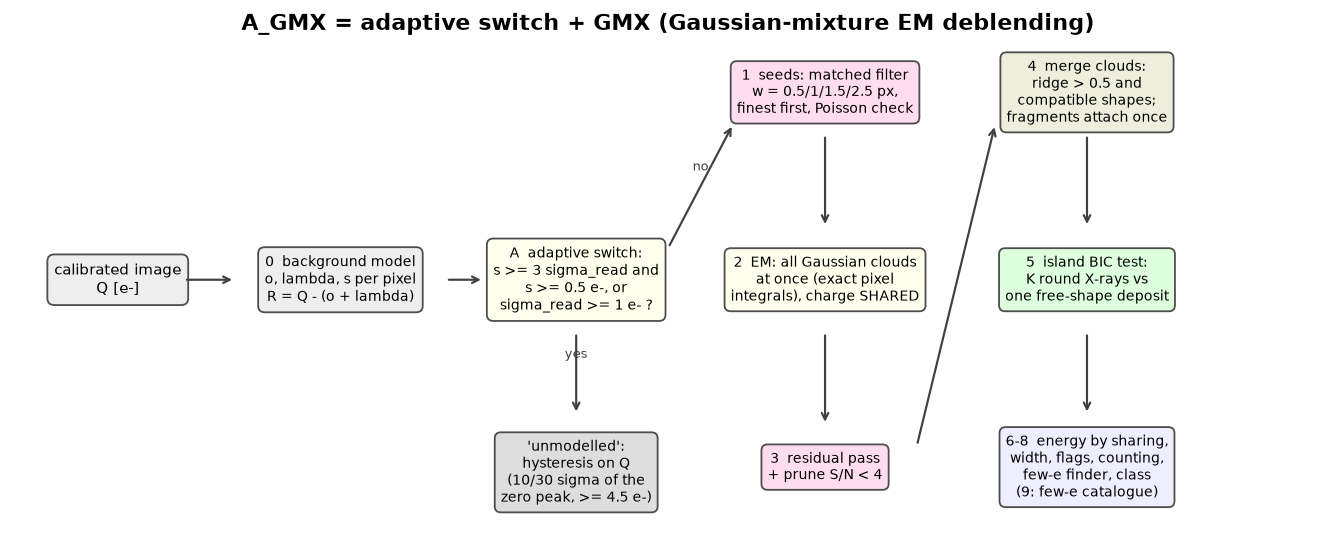
\includegraphics[width=\textwidth]{figures_current/fig00_flowchart.png}
\caption{The steps of \AGMX{} (the numbers refer to the sections below).}
\end{figure}

\begin{figure}[H]\centering
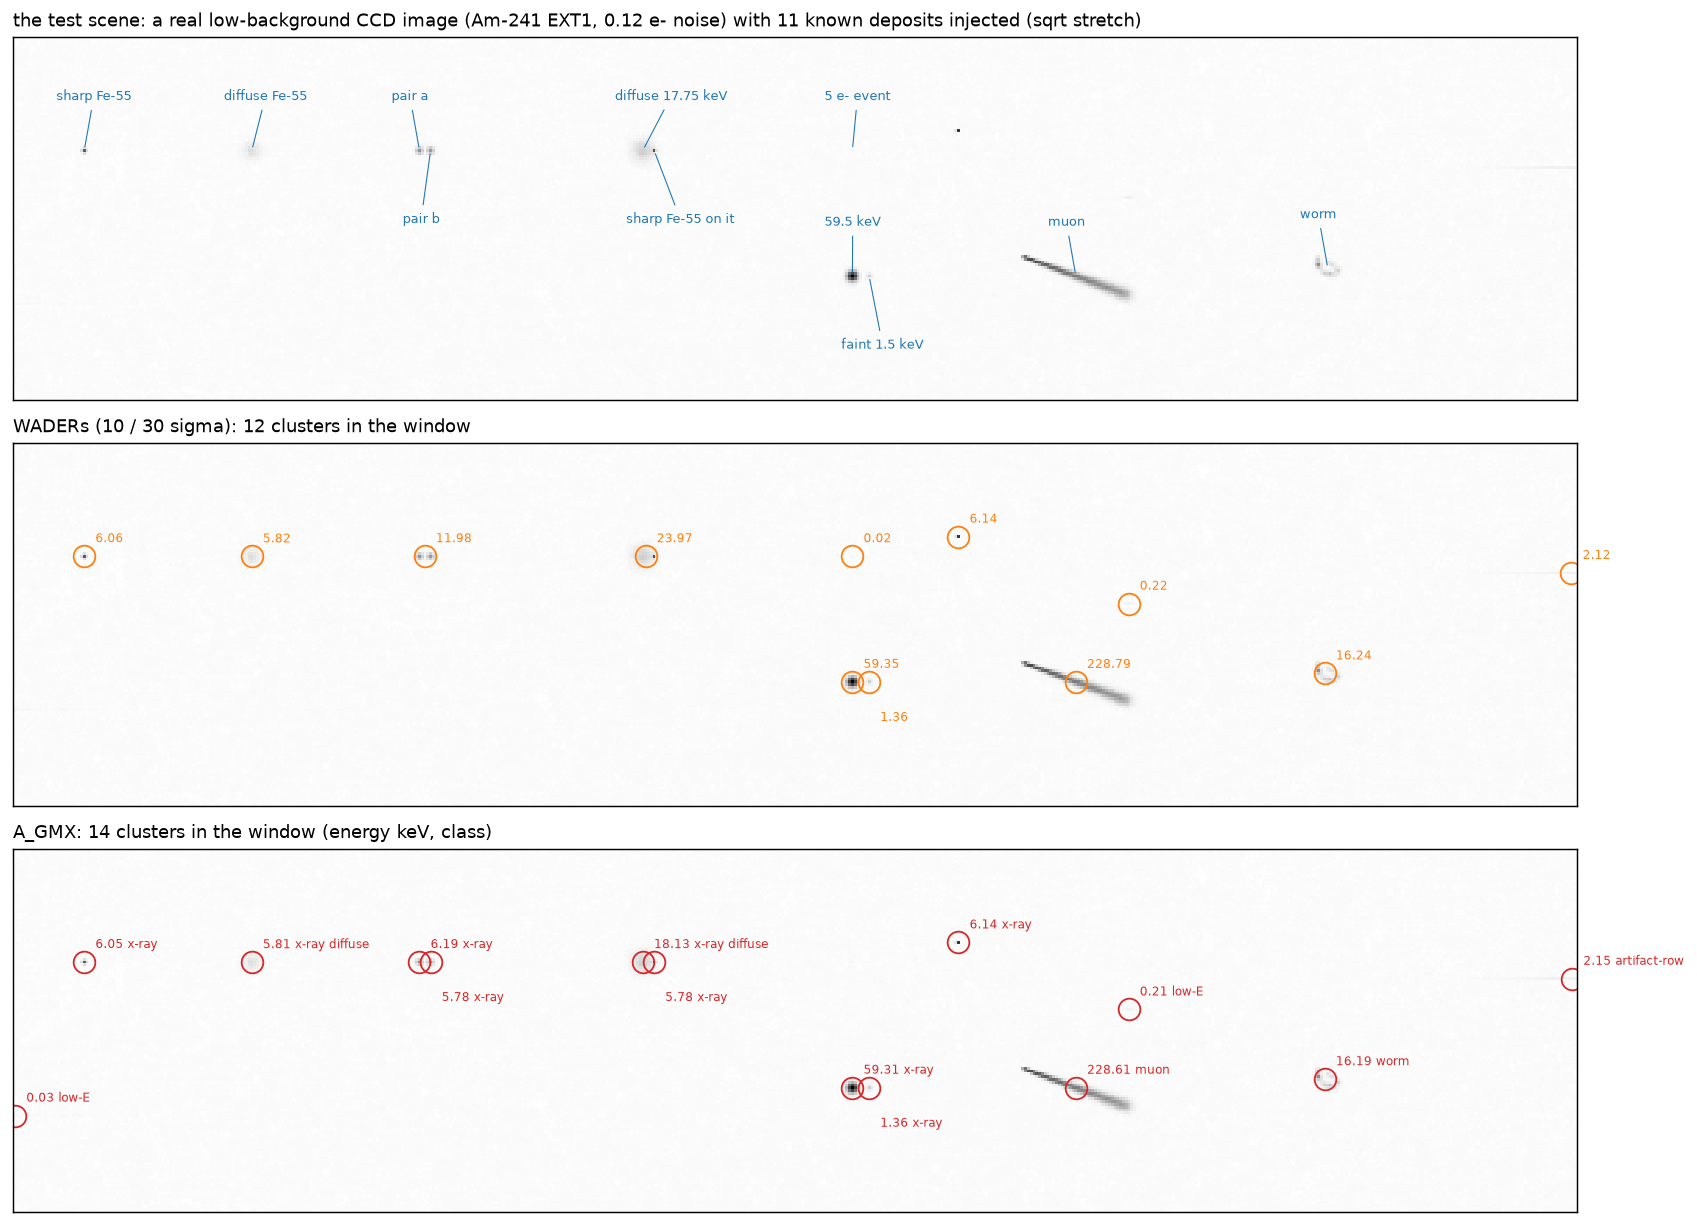
\includegraphics[width=\textwidth]{figures_current/fig01_overview.png}
\caption{A real low-background CCD image (Am-241, EXT1, 0.12\,\el{} read noise) with eleven known deposits injected (top).
WADERs (middle) merges the 4-px pair into one 12-keV cluster and the sharp X-ray sitting on a diffuse one into one 24-keV
cluster. \AGMX{} (bottom) separates both and labels the muon, the worm and the X-rays. Numbers: energies in keV.}
\label{fig:overview}
\end{figure}

%======================================================================================================
\section{The image model and notation}

A calibrated image is a grid of pixel values $Q_p$ in electrons ($p$ = pixel). Each pixel holds
\begin{equation}
Q_p = o_p + n_p + \epsilon_p + D_p, \qquad n_p\sim\mathrm{Poisson}(\lambda_p),\quad \epsilon_p\sim\N(0,s_p^2),
\end{equation}
\begin{itemize}\itemsep0pt
\item $o_p$: offset (where ``0 electrons'' sits after calibration),
\item $n_p$: dark charge, an integer number of electrons, Poisson with mean $\lambda_p$ (\el/pix),
\item $\epsilon_p$: read noise, Gaussian with width $s_p$ (0.1--0.3\,\el{} on skipper CCDs),
\item $D_p$: charge from particle deposits --- what we want.
\end{itemize}
A deposit of charge $A$ (electrons) whose charge cloud has covariance $\Sigma$ (diffusion in the silicon: $\sim$0.1--0.3\,px
on the front side, up to $\sim$1.5\,px on the back side) puts on average
\begin{equation}
D_p = A\int_{\text{pixel }p}\N(\mathbf u;\bm\mu,\Sigma)\,d^2u
\end{equation}
electrons in pixel $p$. Energy = charge $\times$ 3.74\,eV/\el. When the module's gain-versus-charge curve $g(n)$ is
available, the image is converted ADU $\to$ electrons with it \emph{before} \AGMX{} runs (\code{src/agmx\_root.py}), so
shared pixels are split after the nonlinearity is removed.

\begin{table}[H]\centering\small
\begin{adjustbox}{max width=\linewidth}
\begin{tabular}{ll}
\toprule
symbol & meaning \\
\midrule
$R_p = Q_p-(o_p+\lambda_p)$ & residual charge: $\approx0\pm$ noise if empty, $\approx$ deposit charge otherwise \\
$V_p=\lambda_p+s_p^2$ & variance of an empty pixel \\
$R_p^+=\max(R_p,0)$ & the non-negative charge used as weight in the fit \\
$k=1\dots K$ & clouds (components of the mixture) \\
$A_k,\ \bm\mu_k,\ \Sigma_k$ & charge, centre, covariance of cloud $k$ \\
$g_k(p)$ & expected charge of cloud $k$ in pixel $p$ \\
$M_p=\sum_k g_k(p)$ & model of the deposit charge in pixel $p$ \\
\bottomrule
\end{tabular}
\end{adjustbox}
\end{table}

%======================================================================================================
\section{Step 0 --- the background model}\label{sec:bg}

Before looking for deposits, \AGMX{} describes the empty image (\code{agent\_methods.background\_map}). The background is
estimated on the pixels that are not part of deposits, and which pixels those are is found iteratively:

\paragraph{Pass 1: a crude mask.} With the median and the robust spread (MAD) of all active pixels, every pixel above
median $+\max(4\,\el, 5\,\mathrm{MAD})$ is masked and the mask is grown by 5\,px. Most pixels hold 0 or 1 electron, so this
needs no background model; it only has to catch the obvious deposits.

\paragraph{Row fits.} For every row, the unmasked pixels are fitted with the \textbf{Poisson $\otimes$ Gaussian comb}
\begin{equation}
P(Q)=\sum_{n=0}^{\infty}\frac{\lambda^n e^{-\lambda}}{n!}\,\N\!\left(Q;\,o+n,\,s^2\right),
\end{equation}
integer electrons smeared by read noise (figure~\ref{fig:bg}, bottom). The fast fit uses the comb phase
$z=\langle e^{2\pi iQ}\rangle$: the integer Poisson part drops out, so $o=\arg z/2\pi$ and $s=\sqrt{-\ln|z|/2\pi^2}$; $\lambda$ is a
truncated-Poisson fit of the rounded counts $n\le K$ ($K$ a high Poisson quantile, $\ge3$), which ignores leftover cluster
pixels. A row counts as resolved only if $|z|$ exceeds $\max(e^{-2\pi^2 0.45^2},\,4/\sqrt N)$, i.e.\ above the floor
$\sqrt{\pi/4N}$ that $N$ pixels of pure Gaussian noise give. Rounding counts noise above $+0.5$\,\el{} as an electron, so on
these rows $\lambda\leftarrow(\lambda-p)/(1-2p)$ with $p=\Phi^c(0.5/s)$.

\paragraph{Rows without a visible comb.} Where deposits cover most of a row (a charge sheet on a crowded CCD) the comb
cannot be measured; when at least 5\,\% of the rows (and 10 rows) are resolved, such rows take $o$, $\lambda$, $s$ from the
nearest resolved rows (the read noise belongs to the amplifier). Only when almost no row is resolved is a pooled comb
likelihood fitted over groups of 16 rows.

\paragraph{Smoothing.} $\lambda$ and $s^2$ are smoothed along the rows (local-linear, $\pm15$ rows), $o$ is kept per row,
and a 2-D correction from the mean residual in $60\times128$-px cells is added to $\lambda$ (floor $10^{-6}$\,\el/pix).

\paragraph{Pass 2: the calibrated mask.} With this background, a pixel belongs to a deposit when the $3\times3$ box around it
or the pixel alone is unlikely from dark charge and noise (Poisson tail probabilities below $3\times10^{-5}$ and $10^{-5}$;
Poisson, not Gaussian, so the mask does not explode at low dark charge), grown by 4\,px; the row fits are repeated with it.
This mask is used only for the background; the cluster finding below starts from scratch.

This gives per-pixel maps $o_p$, $\lambda_p$, $s_p$ (figure~\ref{fig:bg}, top), hence
\begin{equation}
\mathrm{mean}_p=o_p+\lambda_p,\qquad V_p=\lambda_p+s_p^2,\qquad R_p=Q_p-\mathrm{mean}_p .
\end{equation}

\paragraph{Read noise.} $\sigma_\mathrm{read}=1.4826\times$ the MAD of the pixels with $|Q|<0.5$\,\el; that estimate cannot
exceed $0.37$\,\el{} (a uniform spread), so above 0.3\,\el{} the robust spread of all active pixels is used.

\paragraph{Hot columns.} Per column, the mean of $Q-o-\lambda$ after one $5\sigma$ clip around the column median is compared
with the median of the $\pm10$ neighbouring columns. A column whose excess $d$ is $>5\times$ its error and $>0.05$\,\el{}
gets $\lambda\leftarrow\lambda+d$, so the mean, the variance and the Poisson tests all include it. If more than 10\,\% of the
columns would be flagged the image has a charge sheet, not hot columns, and nothing is flagged.

\begin{figure}[H]\centering
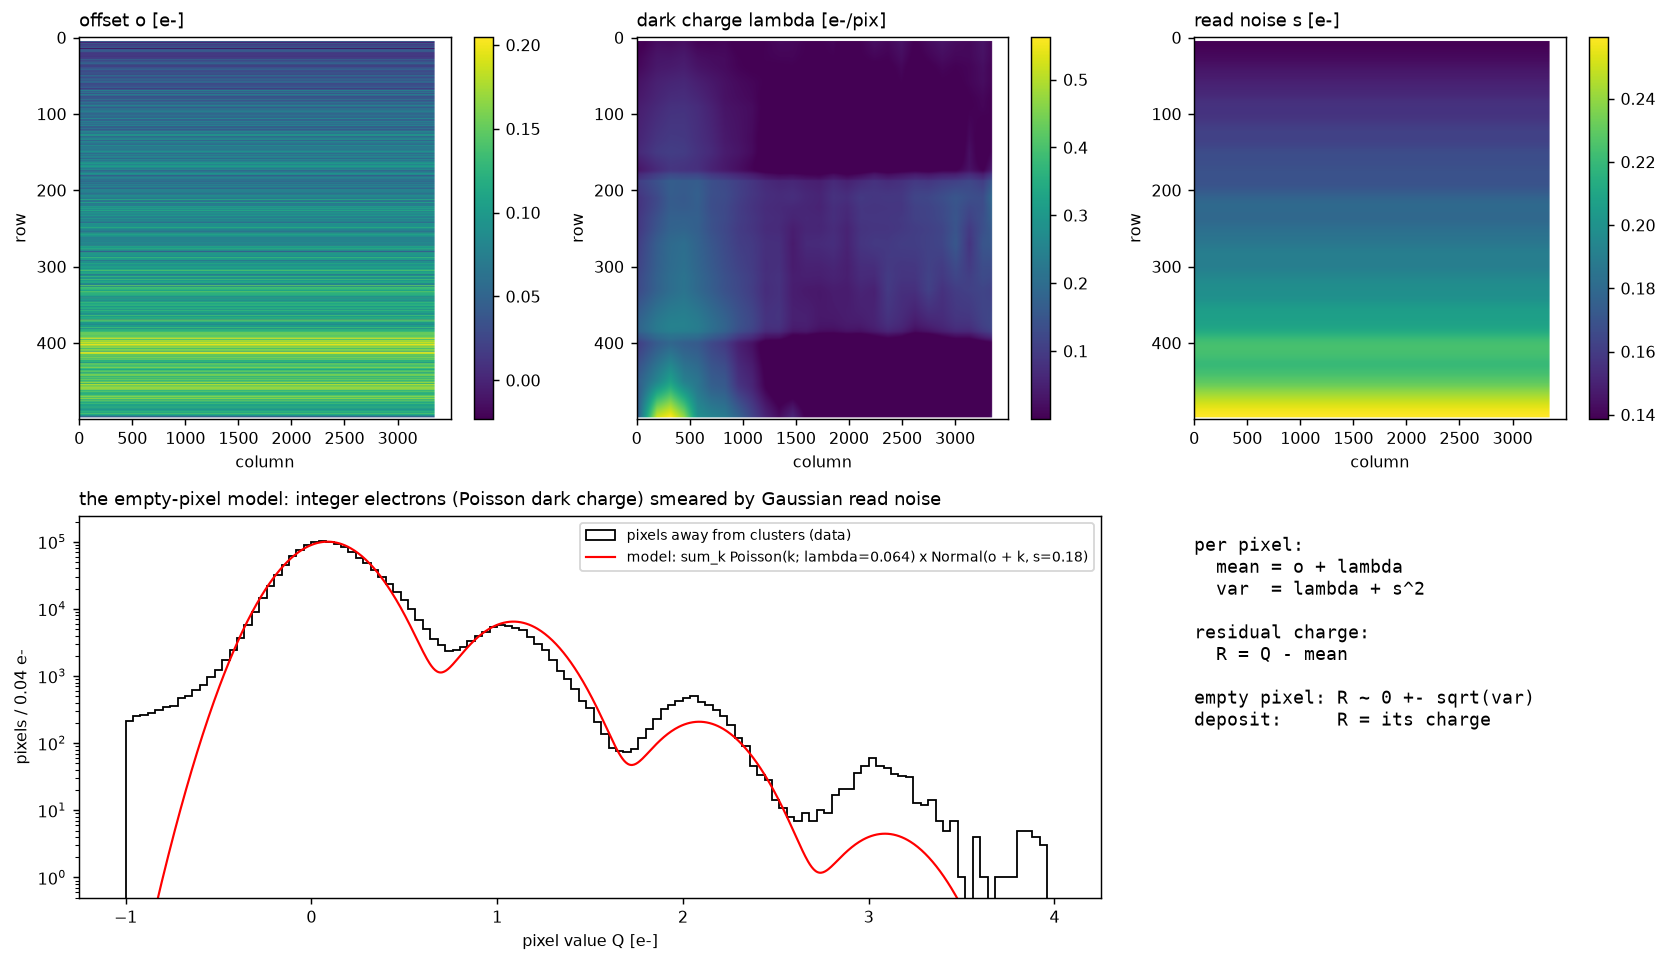
\includegraphics[width=\textwidth]{figures_current/fig02_background.png}
\caption{Top: the fitted offset, dark-charge and read-noise maps of the test image. Bottom: pixels away from clusters (black)
and the comb model (red; drawn with the image's median $\lambda$ and $s$ --- the fit itself is per row, which is why the data's
2- and 3-\el{} peaks lie above a single-$\lambda$ curve).}\label{fig:bg}
\end{figure}

%======================================================================================================
\section{Step A --- the adaptive switch}\label{sec:switch}

The background model can fail: on some images (the PD06/DM12 Am-241 frames) the pixels scatter far more than dark charge +
read noise allow, and every model-based method then measures energies 5--10\,\% high. An image is \textbf{unmodelled} when
\begin{equation}
\boxed{\;\big(s\ge0.5\,\el\ \text{ and }\ s\ge3\,\sigma_\mathrm{read}\big)\ \text{ or }\ \sigma_\mathrm{read}\ge1\,\el\;}
\end{equation}
with $s$ the median fitted noise. The second condition catches images that are not electron-counting at all (with a few
\el{} of noise per pixel the sum over a GMX footprint collects $\sqrt{N_\mathrm{pix}}$ times the noise).

\paragraph{Unmodelled $\to$} hysteresis clustering on the image itself (the model's offset is not trusted either): with
$\sigma_z$ the MAD of the zero-electron peak, pixels above $\max(10\sigma_z,\,4.5\,\el)$ that touch (8 neighbours) form a
cluster, kept if one pixel exceeds $\max(30\sigma_z,\,9.5\,\el)$; energy $=\sum Q_p$.

\paragraph{Otherwise $\to$} GMX on the whole image (steps 1--8). Every cluster also reports the \textbf{event occupancy} of its
$31\times31$-px neighbourhood (fraction of pixels holding event charge; $\ge0.3\to$ ``crowded''); it is information only.

%======================================================================================================
\section{Step 1 --- where are the deposits?}

\subsection{The matched filter}
To decide whether there is a blob of width $w$ centred at pixel $c$, a \textbf{matched filter} is used: a weighted sum of the
residuals with the expected shape as weights. The weights are the fraction of a unit-charge Gaussian cloud of width $w$, centred
on the centre of pixel $c$, that falls in each pixel $p=(i,j)$ --- the exact pixel integral, separable into $y$ and $x$:
\begin{equation}
h_w(p-c)=f(i-c_y)\,f(j-c_x),\qquad f(u)=\tfrac12\Big[\mathrm{erf}\Big(\tfrac{u+\frac12}{\sqrt2\,w}\Big)-\mathrm{erf}\Big(\tfrac{u-\frac12}{\sqrt2\,w}\Big)\Big],
\end{equation}
on a footprint of $\pm\lceil4w+1\rceil$\,px (\code{agent\_methods.\_f1d}). With these weights,
\begin{equation}
S_w(c)=\sum_p h_w(p-c)\,R_p,\qquad \mathrm{Var}[S_w(c)]=\sum_p h_w(p-c)^2V_p,\qquad
\boxed{T_w(c)=\frac{\sum_p h_w(p-c)\,R_p}{\sqrt{\sum_p h_w(p-c)^2\,V_p}}}
\end{equation}
$T_w$ is the significance (in Gaussian sigmas) of a blob of width $w$ at $c$. Summing many pixels with the right weights makes a
deposit far more significant than any single pixel: a 5.9-keV X-ray spread over 20 pixels is invisible to a per-pixel
$10\sigma$ threshold in its tails but has $T\gg100$. Both sums are separable convolutions (\code{gmx.\_sep\_conv}),
computed for four widths $w\in\{0.5,1,1.5,2.5\}$\,px (sharp front-side X-rays to diffuse back-side ones and blobs).

\paragraph{Normalisation and optimality.} The overall scale of $h_w$ cancels in $T_w$. Because the denominator is the exact
standard deviation of the numerator for an empty region, $T_w$ is a correctly normalised significance even where the noise
varies from pixel to pixel. For noise that is the same in every pixel the filter is the optimal linear detector (largest
signal-to-noise for a known shape; Turin 1960). Where $V_p$ varies across the footprint (hot columns, steep dark-charge
gradients) the optimal filter would also weight each pixel by $1/V_p$,
$T^{\mathrm{opt}}_w=\sum_p h_w R_p/V_p\,\big/\sqrt{\sum_p h_w^2/V_p}$; the unweighted numerator used here loses a little
sensitivity there but keeps the false-alarm rate correct. At very low dark charge the noise is Poisson rather than Gaussian,
and the optimal Poisson template statistic is $\sum_p n_p\ln(1+h_wA/B_p)$ ($n_p$ the counts, $A$ the deposit charge, $B_p$ the
background; Ofek \& Zackay 2018); this is why every seed must also pass the exact Poisson box test below. The template sits on
the pixel centre only (no sub-pixel offset): the EM fit of step~2 finds the centre.

\subsection{Scale-space seeds}
Seeds are local maxima ($5\times5$, over valid pixels only) with $T_w>5$. The scales are visited \textbf{finest first}; a
maximum at a coarser scale is kept only if no finer-scale seed lies within $\max(2,1.5w)$\,px; within a scale, seeds closer
than that are suppressed (greedy, strongest first). Why: two X-rays 4--5\,px apart give two maxima at $w=0.5$ but one merged
maximum in the middle at $w=2.5$; finest-first keeps the two (scale-space detection, Lindeberg 1994). A lone diffuse X-ray has
no fine-scale maximum (its peak is too flat), so its coarse-scale seed survives.

\begin{figure}[H]\centering
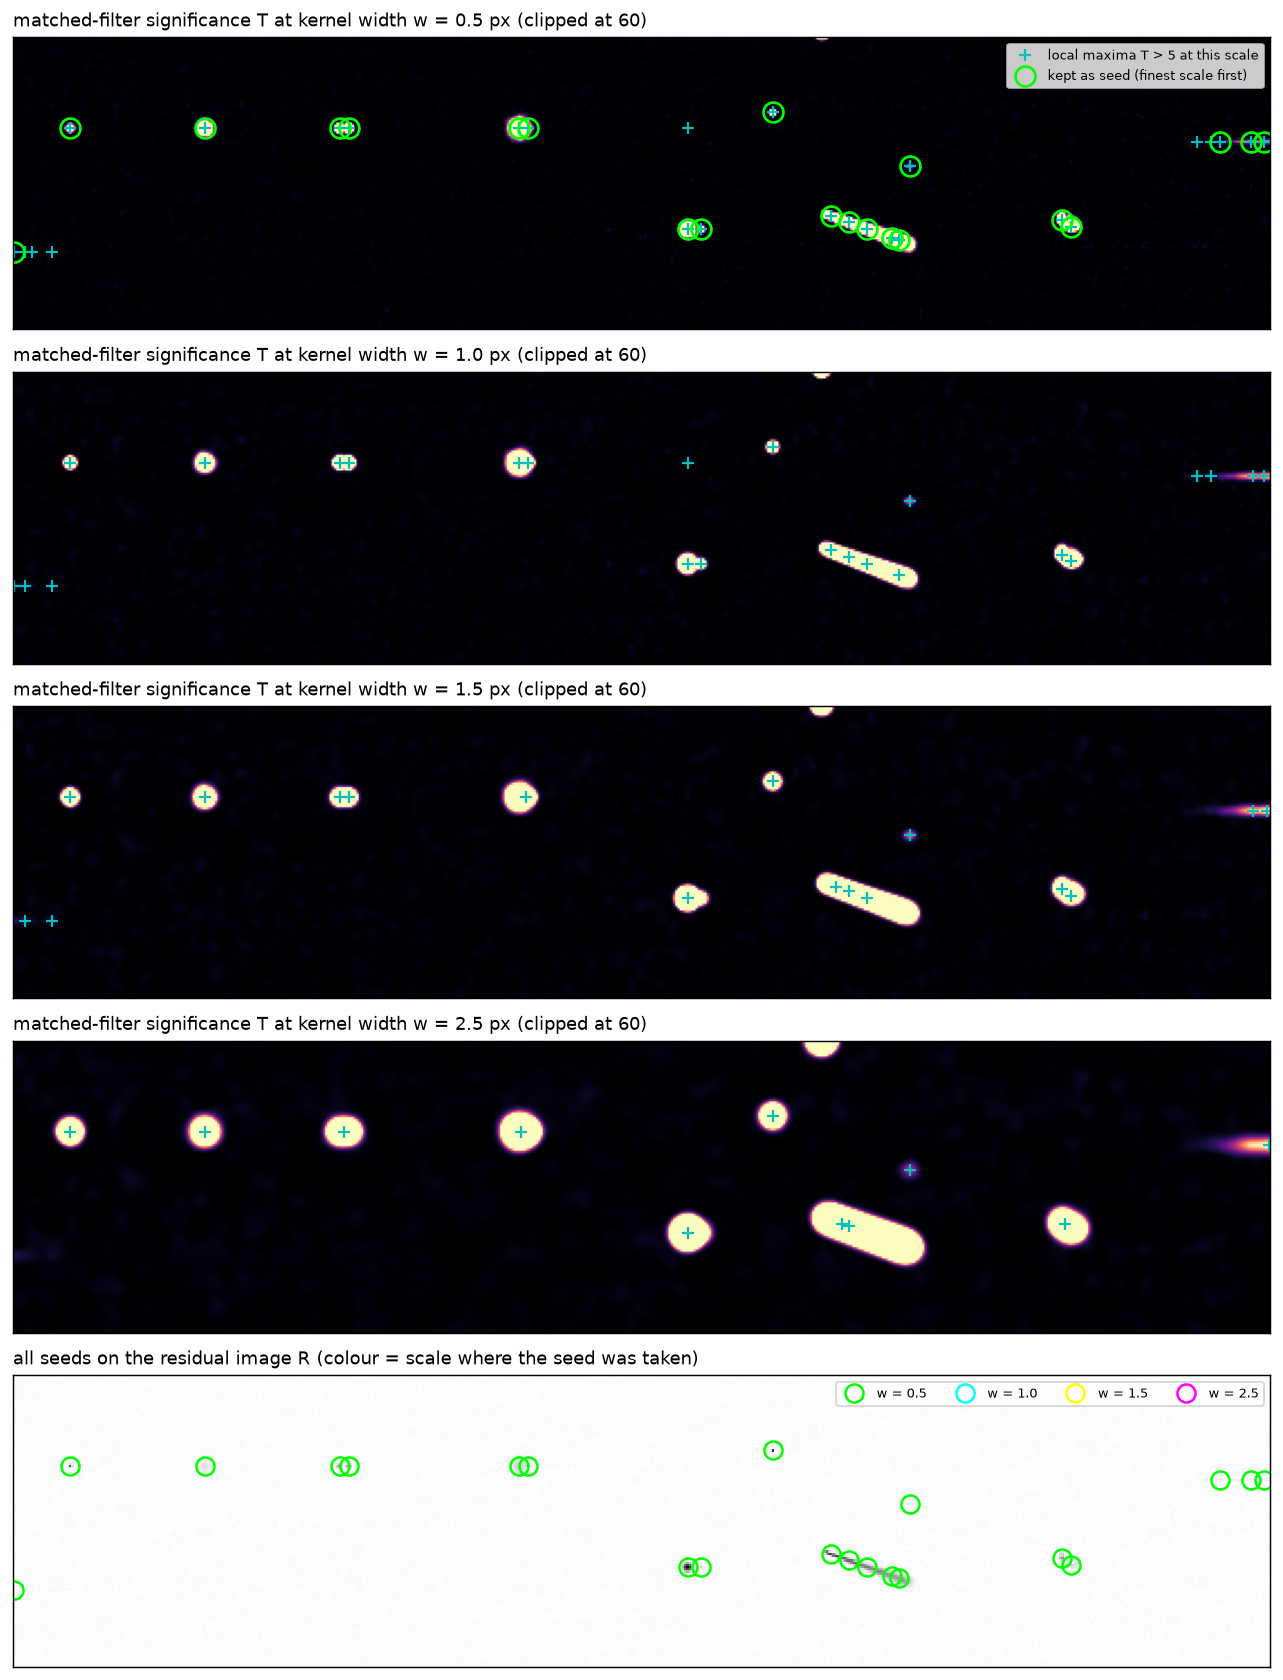
\includegraphics[width=0.95\textwidth]{figures_current/fig03_matched_filter_seeds.png}
\caption{$T_w$ at the four widths (clipped at 60) with the local maxima (+) and the seeds kept (circles). Bottom: all seeds on
$R$, coloured by the scale they were taken at. The 4-px pair and the sharp X-ray on the diffuse one get two seeds each; the
muon and the worm get several.}
\end{figure}

\subsection{The Poisson check}
$T_w$ treats the noise as Gaussian, but dark charge is integer and Poisson: at low $\lambda$ a lone box of 3 electrons is
``$6\sigma$'' in Gaussian terms but has probability $\sim10^{-4}$ (figure~\ref{fig:poisson}). Every seed must therefore also
pass an \textbf{exact counting test} on the $3\times3$ or the $5\times5$ box around it (the idea of Li \& Ma 1983 in
$\gamma$-ray astronomy): with $S=\sum_\mathrm{box}(Q_p-o_p)$, $\Lambda=\sum_\mathrm{box}\lambda_p$,
$\sigma_\mathrm{box}=\sqrt{\sum_\mathrm{box}s_p^2}$,
\begin{equation}
P\!\left(\mathrm{Poisson}(\Lambda)\ \ge\ \lfloor S-2\sigma_\mathrm{box}+0.5\rfloor\right)<\Phi^c(5)=2.9\times10^{-7}.
\end{equation}
The $-2\sigma_\mathrm{box}$ term protects against read noise pushing a box up by a fraction of an electron. On
electron-counting CCDs $\lambda$ here is the detection dark charge of step~7.

\begin{figure}[H]\centering
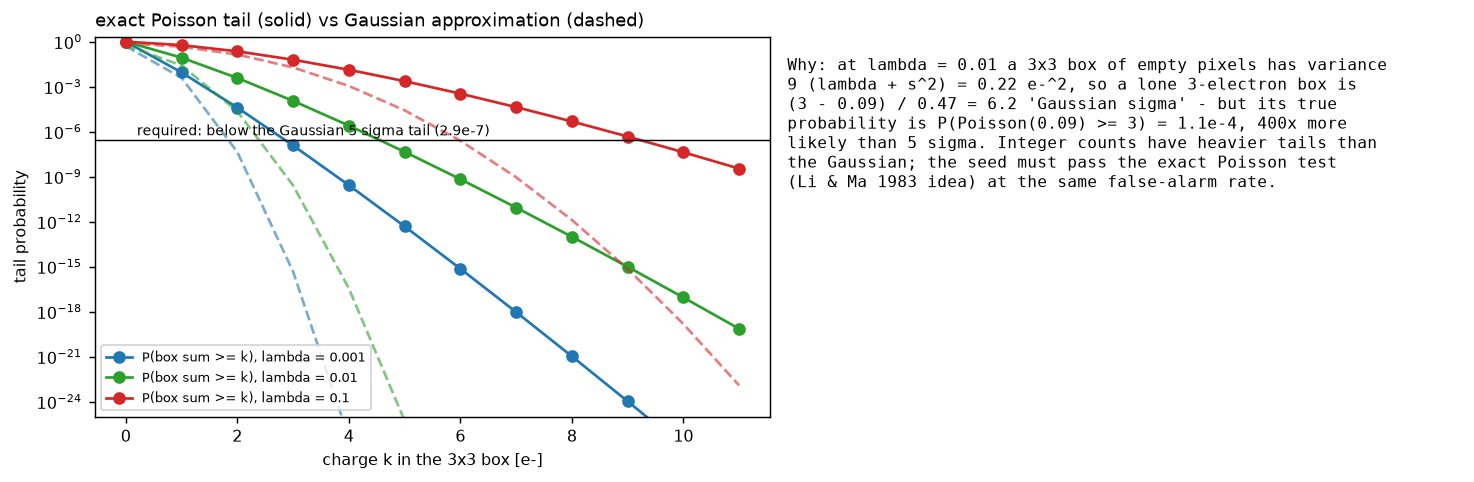
\includegraphics[width=0.9\textwidth]{figures_current/fig04_poisson_check.png}
\caption{Tail probability of the $3\times3$-box charge from dark current alone: exact Poisson (solid) versus the Gaussian
approximation (dashed). At low dark charge the Gaussian approximation is far too optimistic; the seed has to be below the
horizontal line in the exact calculation.}\label{fig:poisson}
\end{figure}

Each surviving seed starts a round cloud: $\bm\mu$ = the seed pixel, $\Sigma=w^2\mathbf 1$ ($w$ = scale of the seed) and
$A_0=\max\!\big(R_\mathrm{peak}\cdot2\pi(w^2+\tfrac1{12}),\,1\big)$ (the charge of a Gaussian with that peak height).

%======================================================================================================
\section{Step 2 --- fitting all deposits at once}

\subsection{The model}
\begin{equation}
M_p=\sum_{k=1}^{K}g_k(p).
\end{equation}
Each cloud has its own charge $A_k$, centre $\bm\mu_k$ and \textbf{full} covariance
$\Sigma_k=\begin{pmatrix}\sigma_{yy}&\sigma_{xy}\\ \sigma_{xy}&\sigma_{xx}\end{pmatrix}$, so it can be round (an X-ray) or
elliptical and tilted (a piece of a track). For a cloud with correlation $|\rho|=|\sigma_{xy}|/\sqrt{\sigma_{yy}\sigma_{xx}}<0.5$
(every X-ray) the model value is the \textbf{exact integral of the Gaussian over the pixel}:
\begin{equation}
g_k(p)=A_k\Big[\Phi\big(\tfrac{i+\frac12-\mu_{y}}{\sigma_{y}}\big)-\Phi\big(\tfrac{i-\frac12-\mu_{y}}{\sigma_{y}}\big)\Big]
\Big[\Phi\big(\tfrac{j+\frac12-\mu_{x}}{\sigma_{x}}\big)-\Phi\big(\tfrac{j-\frac12-\mu_{x}}{\sigma_{x}}\big)\Big].
\end{equation}
This matters for sharp clusters: a 0.2-px cloud puts almost all its charge in one or two pixels, and a Gaussian evaluated at
the pixel centre would predict a peak that is too high and tails that are too low. Strongly correlated clouds (pieces of tilted
tracks, broad along the track) use $A_k\,\N(\mathbf x_p;\bm\mu_k,\Sigma_k+\tfrac1{12}\mathbf 1)$, the Gaussian at the pixel centre
with the variance of a uniform pixel added. Each cloud is evaluated only within its $4\sigma$ ellipse (at least 2\,px, at most
16\,px), as sparse arrays.

\subsection{What is maximised}
Treat the deposit charge as \textbf{counts} with mean $M_p+\varepsilon_p$, where $\varepsilon_p=\sqrt{V_p}$ is a fixed
``unexplained'' level per pixel (a noise component of the mixture). The Poisson log-likelihood is
\begin{equation}
\ln L=\sum_p\Big[R_p^+\ln\big(M_p+\varepsilon_p\big)-\big(M_p+\varepsilon_p\big)\Big].
\end{equation}
Maximising it over $\{A_k,\bm\mu_k,\Sigma_k\}$ is a missing-data problem: if we knew which cloud each electron came from, each
cloud could be fitted alone. \textbf{Expectation--maximisation} (Dempster, Laird \& Rubin 1977; for Poisson images Shepp \&
Vardi 1982, Richardson 1972, Lucy 1974) alternates two steps. For the amplitudes with the shapes held fixed, the update
$A_k\leftarrow\sum_p r_{pk}R_p^+$ is the classic ML-EM (Richardson--Lucy) step and never decreases $\ln L$; the centre and
covariance updates are the weighted-moment M-step of a Gaussian mixture. With the safeguards below monotonic convergence is
not guaranteed in general, but the \textbf{cluster energies}, which share the measured charge, are stable: 60 instead of 30
iterations changes X-ray cluster energies by $<0.004\,\%$ (99th percentile). Running EM to convergence (centre steps
$<0.01$\,px) was tested on the crowded CCD and gave no consistent gain, so a fixed number of iterations is used.

\subsection{E-step: who owns each pixel?}
\begin{equation}
\boxed{\;r_{pk}=\frac{g_k(p)}{M_p+\varepsilon_p}\;}\qquad
\Big(\textstyle\sum_k r_{pk}+\frac{\varepsilon_p}{M_p+\varepsilon_p}=1\Big)
\end{equation}
$r_{pk}$ is the expected fraction of pixel $p$'s charge that came from cloud $k$ (its \textbf{responsibility}). The noise
share $\varepsilon_p/(M_p+\varepsilon_p)$ is $\approx1$ far from every cloud, so noise pixels are not handed to any cloud
(figure~\ref{fig:resp}, right, dotted).

\subsection{M-step: update each cloud from its share}
The E-step gives every cloud a share of every pixel in its footprint, $w_{pk}=r_{pk}R_p^+$ (the charge of pixel $p$ attributed to
cloud $k$). The M-step re-estimates each cloud from its own share alone, in four steps. Pixel $p$ sits at integer coordinates
$\mathbf x_p=(i_p,j_p)$ (pixel centres).

\paragraph{1. Charge.} The cloud's charge is the total charge it was given:
\begin{equation}
A_k=\sum_p w_{pk}.
\end{equation}

\paragraph{2. Moments of the share.} The charge-weighted mean position and the charge-weighted (co)variances of the pixels of the
share are
\begin{equation}
\bar y_k=\frac{1}{A_k}\sum_p w_{pk}\,i_p,\qquad \bar x_k=\frac{1}{A_k}\sum_p w_{pk}\,j_p,
\end{equation}
\begin{equation}
v^{yy}_k=\frac{1}{A_k}\sum_p w_{pk}(i_p-\bar y_k)^2,\qquad
v^{xx}_k=\frac{1}{A_k}\sum_p w_{pk}(j_p-\bar x_k)^2,\qquad
v^{xy}_k=\frac{1}{A_k}\sum_p w_{pk}(i_p-\bar y_k)(j_p-\bar x_k).
\end{equation}
These are the moments of a \emph{pixelised} cloud (charge collected in whole pixels), not yet the moments of the physical charge
cloud: pixelisation shifts the mean towards the nearest pixel centre and changes the variance, by an amount that depends on the
cloud's width and on where its centre sits inside the pixel.

\paragraph{3. From the pixelised moments to the physical cloud.} For an uncorrelated cloud ($|\rho|<0.5$, the exact pixel model
of step~2) the two axes separate. Along one axis, a Gaussian of variance $\sigma^2$ centred at offset $\delta$ from a pixel centre
puts the fraction
\begin{equation}
\pi_i(\sigma^2,\delta)=\Phi\Big(\frac{i+\frac12-\delta}{\sigma}\Big)-\Phi\Big(\frac{i-\frac12-\delta}{\sigma}\Big)
\end{equation}
of its charge in pixel $i$. Its pixelised mean and variance are
\begin{equation}
\mathcal M(\delta,\sigma^2)=\sum_i i\,\pi_i,\qquad \mathcal V(\sigma^2,\delta)=\sum_i\big(i-\mathcal M\big)^2\pi_i .
\end{equation}
Two examples show why this matters: a $\sigma=0.2$\,px cloud has $\mathcal V=0.01$\,px$^2$ when centred on a pixel ($\delta=0$)
but $0.25$\,px$^2$ when centred on a pixel edge ($\delta=0.5$, the charge splits between two pixels); and its pixelised mean is
pulled towards the pixel centre. The M-step inverts these functions, per axis:
\begin{equation}
\sigma_{yy,k}=\mathcal V^{-1}\big(v^{yy}_k\,\big|\,\delta=\mathrm{frac}(\mu_{y,k}^\mathrm{old})\big),\qquad
\mu_{y,k}=\lfloor\bar y_k\rceil+\mathcal M^{-1}\big(\bar y_k-\lfloor\bar y_k\rceil\,\big|\,\sigma_{yy,k}\big),
\end{equation}
and the same for $x$ ($\lfloor\cdot\rceil$: the nearest integer; $\mathrm{frac}$: the distance of the previous centre from its
nearest pixel centre, 0--0.5). The variance is inverted at the previous centre's sub-pixel offset, then the mean at the new
variance. $\mathcal V$ and $\mathcal M$ are tabulated once (\code{gmx.\_pixvar\_table}: 26 offsets $\delta\in[0,0.5]$ $\times$ 300
values $\sigma^2\in[10^{-3},30]$\,px$^2$ on a log grid; \code{\_pixmean\_table}: 101 offsets $\in[-0.5,0.5]$ $\times$ 120 values),
summing $\pi_i$ over $i=-40\dots40$, made monotonic in $\sigma^2$, and inverted by linear interpolation. The covariance term
$\sigma_{xy,k}=v^{xy}_k$ is kept: the exact product model of step~2 does not use it, but it decides whether the cloud is
correlated ($|\rho|$) and enters the merging tests of step~4.

For a strongly correlated cloud ($|\rho|\ge0.5$, a piece of a tilted track, modelled as a Gaussian at the pixel centre with the
variance of a uniform pixel added) the inversion is simply
\begin{equation}
\bm\mu_k=(\bar y_k,\bar x_k),\qquad
\Sigma_k=\begin{pmatrix}v^{yy}_k-\tfrac1{12}&v^{xy}_k\\ v^{xy}_k&v^{xx}_k-\tfrac1{12}\end{pmatrix}.
\end{equation}

\paragraph{4. Safeguards.} Variances are clipped to $[0.02,25]$\,px$^2$ and the correlation to
$|\sigma_{xy}|\le0.95\sqrt{\sigma_{yy}\sigma_{xx}}$ (the covariance stays positive definite); a centre moves at most 1.5\,px per
iteration (larger steps are shortened along their direction), which stops a cloud from jumping onto a neighbour; clouds with
$A_k<10^{-3}$\,\el{} are removed. The moments are taken over the cloud's footprint ($4\sigma$ ellipse, at least 2\,px), so the
far tails beyond it are ignored; for a Gaussian that is $<0.1\,\%$ of the charge.

E- and M-step are repeated 30 times. The iteration is compiled (numba); the numpy version (\code{AGMX\_NUMBA=0}) gives identical
results.

\subsection{Why this is the heart of \AGMX}\label{sec:heart}
\textbf{No threshold decides which pixel belongs to which cluster.} Where two deposits overlap, each pixel's charge is split in
proportion to what each cloud predicts there --- this is the \emph{deblending}. Three consequences:
\begin{enumerate}
\item \textbf{No percolation.} In a crowded field, threshold-and-connect methods chain neighbours into one blob (or need such
high thresholds that tails are cut). Sharing has no such failure mode: this is why \AGMX{} beats WADERs on the crowded Am-241 CCD.
\item \textbf{No charge stealing.} A sharp X-ray on the shoulder of a diffuse one keeps only its own charge (figure~\ref{fig:resp}).
\item \textbf{Tails are kept.} The faint tail of a diffuse cluster is explained by its Gaussian, not cut by a threshold: energies
are unbiased at every width (figure~\ref{fig:fe55}) and the back side of Fe-55 sits at the front-side energy.
\end{enumerate}

\begin{figure}[H]\centering
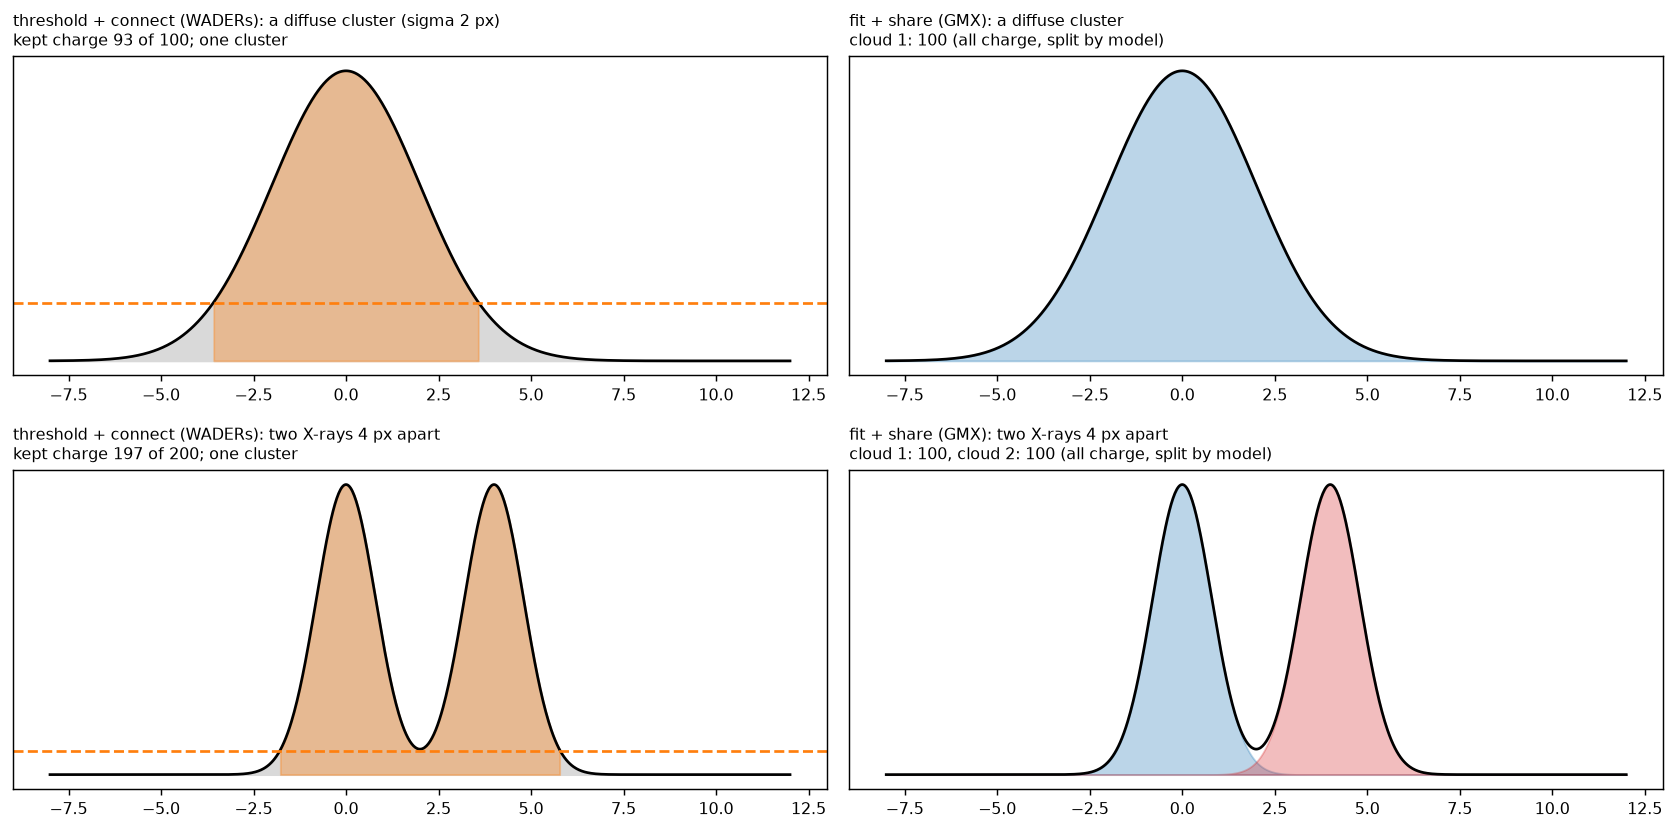
\includegraphics[width=0.85\textwidth]{figures_current/fig12_threshold_vs_sharing.png}
\caption{The difference in one dimension. Left, threshold + connect: the tails of a diffuse cluster below the threshold are lost
and two X-rays 4\,px apart are connected into one cluster. Right, fit + share: every electron is kept and the overlap region is
split between the two clouds in proportion to their predicted charge.}
\end{figure}

\begin{figure}[H]\centering
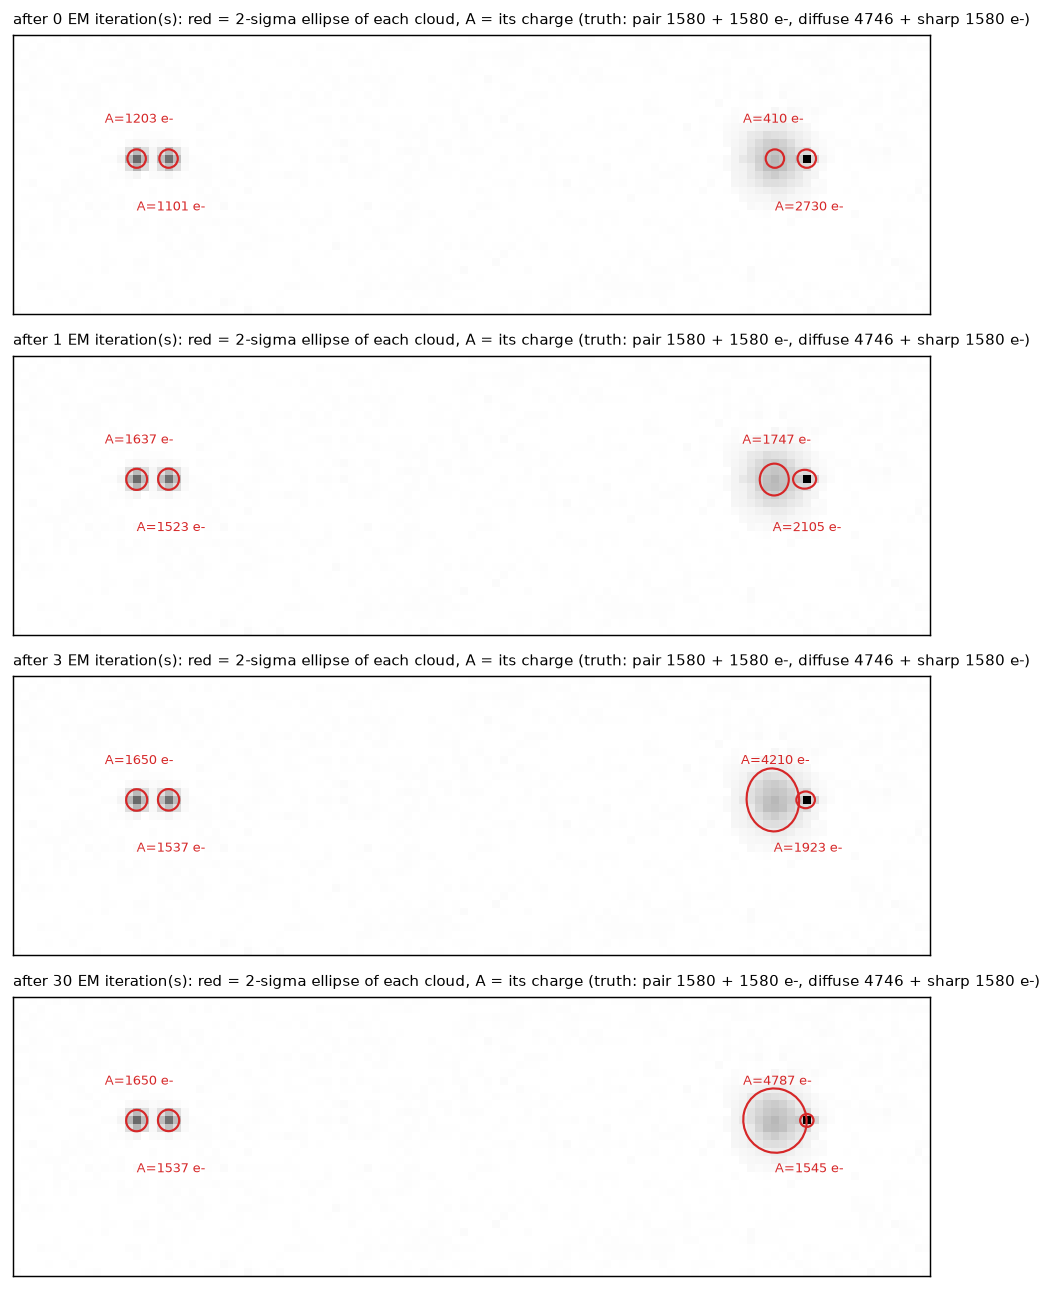
\includegraphics[width=0.75\textwidth]{figures_current/fig05_em_evolution.png}
\caption{EM on the 4-px pair (left) and the sharp X-ray on a diffuse one (right): $2\sigma$ ellipses and charges $A$ after 0, 1,
3 and 30 iterations. The diffuse cloud grows to its width, the sharp one shrinks onto its pixel; final charges 1650 + 1537\,\el{}
and 4787 + 1545\,\el{} (nominal 1580 + 1580 and 4746 + 1580; the injected numbers are Poisson draws).}
\end{figure}

\begin{figure}[H]\centering
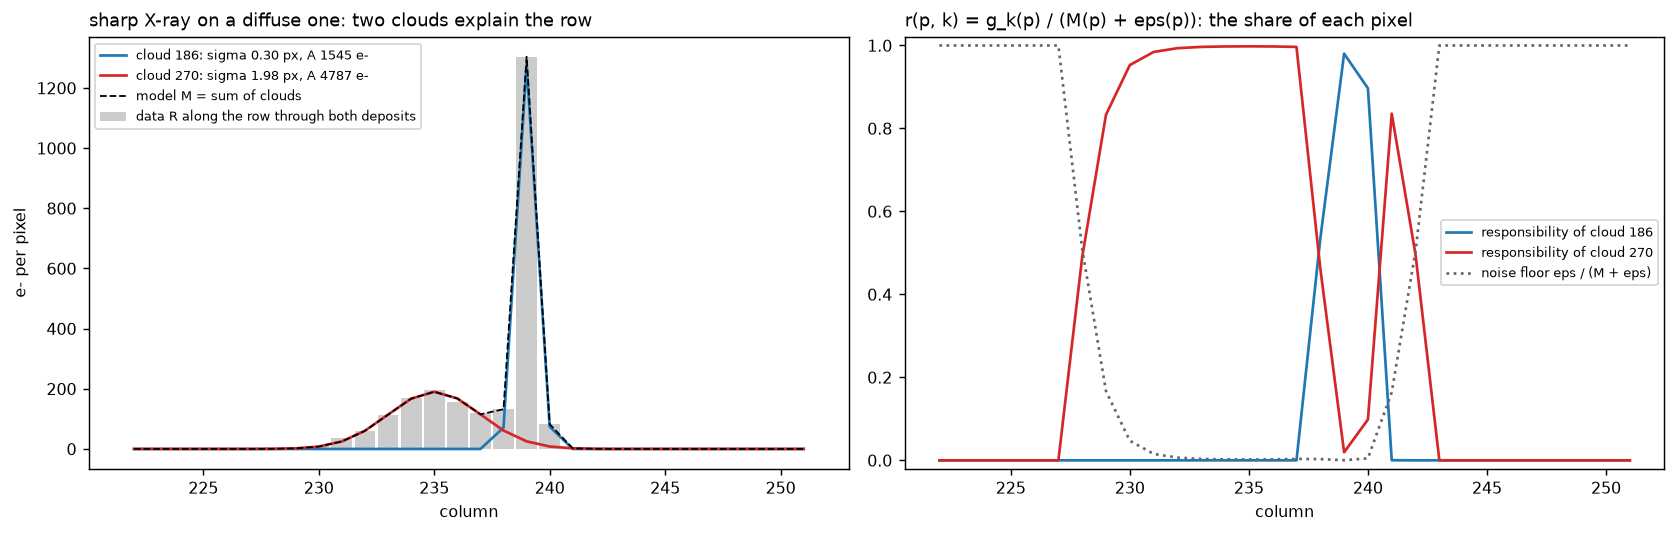
\includegraphics[width=\textwidth]{figures_current/fig06_responsibilities.png}
\caption{Left: the row through the sharp X-ray on the diffuse one --- data (grey), the two clouds ($\sigma$ 0.30 and 1.98\,px)
and their sum. Right: responsibilities; each pixel's charge is split between the two clouds, and far from both the noise share
is $\sim$1.}\label{fig:resp}
\end{figure}

%======================================================================================================
\section{Step 3 --- residual pass and pruning}

\paragraph{Residual pass.} A faint deposit right next to a bright one can be hidden at the seed stage. After EM, the matched
filter is run on the residual $R-M$ with the model's own Poisson variance added, $V'_p=V_p+M_p$, at the two finest scales;
local maxima ($3\times3$) with $T>5$ that pass the Poisson check (counting CCDs) and lie more than 1\,px from any cloud become
new clouds, and EM runs 15 more iterations on all clouds (figure~\ref{fig:resid}).

\paragraph{Pruning.} The significance of cloud $k$ is its charge divided by the uncertainty of that charge. For a linear fit
of $A_k$ with known profile $\pi_k(p)=g_k(p)/A_k$ and per-pixel variance $v_p$ (read noise + dark charge + the other clouds'
model, i.e.\ the variance if this cloud were absent), the Fisher information is $\sum_p\pi_k(p)^2/v_p$, so
\begin{equation}
\mathrm{S/N}_k=A_k\sqrt{\sum_p\frac{\pi_k(p)^2}{V_p+\big(M_p-g_k(p)\big)}} .
\end{equation}
Clouds with $\mathrm{S/N}<4$ are dropped; EM runs 5 more iterations.

\begin{figure}[H]\centering
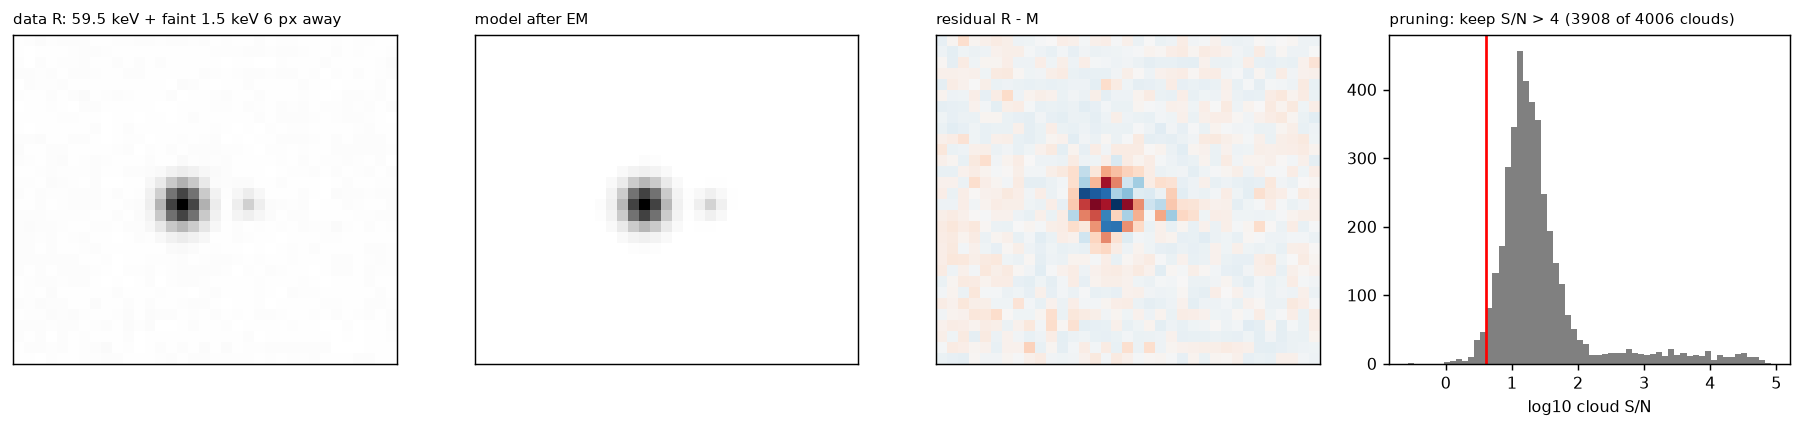
\includegraphics[width=\textwidth]{figures_current/fig07_residual_pruning.png}
\caption{A 59.5-keV X-ray with a faint 1.5-keV X-ray 6\,px away: data, model after the first EM, residual (the faint one stands
out), and the S/N of all clouds of the image with the pruning cut (3908 of 4006 clouds kept).}\label{fig:resid}
\end{figure}

%======================================================================================================
\section{Step 4 --- which clouds are one deposit?}

One deposit can need several clouds (a track needs many; a non-Gaussian X-ray may need two). Clouds are grouped by testing
every pair closer than $3.5(\bar\sigma_i+\bar\sigma_j)+1$\,px ($\bar\sigma$ = geometric-mean width, at most 16\,px).

\paragraph{Ridge (dip) test.} Walk the straight line between the two centres, $\mathbf x(t)=\bm\mu_i+t(\bm\mu_j-\bm\mu_i)$,
$t\in[0,1]$, and evaluate the two-cloud density $f(t)=g_i(\mathbf x(t))+g_j(\mathbf x(t))$ at 17 points:
\begin{equation}
\rho_{ij}=\frac{\min_{t\in[0,1]}f(t)}{\min\big(f(0),f(1)\big)} .
\end{equation}
$\rho\approx1$: no valley, one connected object. $\rho\ll1$: two separate peaks. Required: $\rho>0.5$ (the modality criterion
for merging mixture components; Ray \& Lindsay 2005, Hennig 2010).

\paragraph{Shape test.} Even without a dip, two clouds are merged only if \textbf{one} of these holds:
\begin{itemize}\itemsep0pt
\item similar widths: $\max(\bar\sigma_i,\bar\sigma_j)/\min(\bar\sigma_i,\bar\sigma_j)<1.6$;
\item a track: one cloud is elongated (axis ratio $>1.4$) \textbf{and} its long axis points along the line joining them ($|\cos|>0.8$);
\item a shoulder: the narrower cloud is not a local maximum of $f$ (it only shapes the flank of the broad one).
\end{itemize}
The case this protects: a \textbf{sharp X-ray on top of a diffuse one} is a maximum of its own with a very different width ---
kept apart.

\paragraph{Fragments.} A cloud below 50\,\el{} \emph{and} below 10\,\% of the charge of its brightest merge partner (a few
electrons in the tail of a large deposit, often fitted as a thin ``track'') links only to that partner. It can be part of a
cluster but cannot connect two: without this rule such a fragment linked an X-ray to the big deposit next to it. Pairs that
pass are linked; the connected components of the links are the clusters.

\begin{figure}[H]\centering
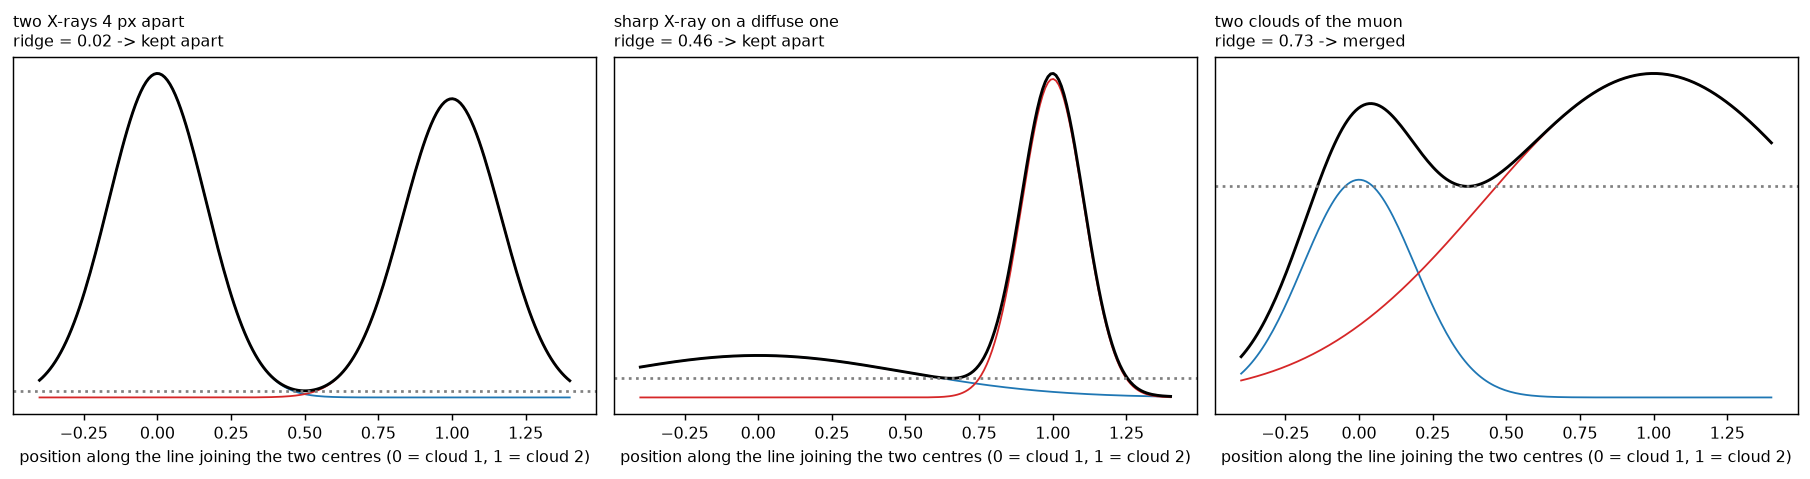
\includegraphics[width=\textwidth]{figures_current/fig08_ridge_test.png}
\caption{Two-cloud density along the line between centres. Left: two X-rays 4\,px apart, deep valley ($\rho=0.02$), kept apart.
Middle: sharp X-ray on a diffuse one --- $\rho=0.46<0.5$, kept apart (it is also a maximum of its own with a very different
width). Right: two clouds of the muon, $\rho=0.73$, merged.}
\end{figure}

%======================================================================================================
\section{Step 5 --- tracks versus several X-rays}

Lumpy electron tracks (``worms'') have real dips along them (their d$E$/d$x$ fluctuates), so the ridge test alone can split them.
The \textbf{island test} asks the data directly.

\textbf{Islands} are connected regions (8 neighbours) of pixels above the Poisson-tail threshold of the dark charge at
$\alpha=0.01$. An island of at most 4000\,px that holds $K\ge2$ clusters (from step 4) is fitted with two hypotheses on its
pixels (+2 rings):
\begin{itemize}
\item $H_\mathrm{xr}$: \textbf{$K$ separate X-rays} --- one \emph{round} Gaussian per cluster (started from the cluster's clouds,
refitted by EM with $\Sigma=\sigma^2\mathbf 1$): 4 parameters each ($A,y,x,\sigma$);
\item $H_\mathrm{free}$: \textbf{one irregular deposit} --- the free-shape clouds already fitted: 6 parameters each
($A,y,x,\sigma_{yy},\sigma_{xx},\sigma_{xy}$), $n_c$ clouds.
\end{itemize}
Each is scored with a weighted $\chi^2$ and the \textbf{Bayesian information criterion} (Schwarz 1978), which charges $\ln n$
per parameter ($n$ = pixels):
\begin{equation}
\chi^2_H=\sum_p\frac{\big(R_p-M_p^{H}\big)^2}{V_p+R_p^++(0.05\,R_p)^2},\qquad
\Delta\mathrm{BIC}=\big(\chi^2_\mathrm{xr}+4K\ln n\big)-\big(\chi^2_\mathrm{free}+6n_c\ln n\big).
\end{equation}
The $(0.05R)^2$ term tolerates the fact that real X-rays are not perfect Gaussians (5\,\% model error). If
$\Delta\mathrm{BIC}>100$ --- the free-shape description is so much better that it is worth its extra parameters --- \textbf{the
whole island becomes one deposit}. The margin of 100 is calibrated on simulated sharp-on-diffuse scenes with the exact pixel
model. In crowded areas islands percolate beyond 4000\,px and the test switches itself off (there, sharing does the work).

\begin{figure}[H]\centering
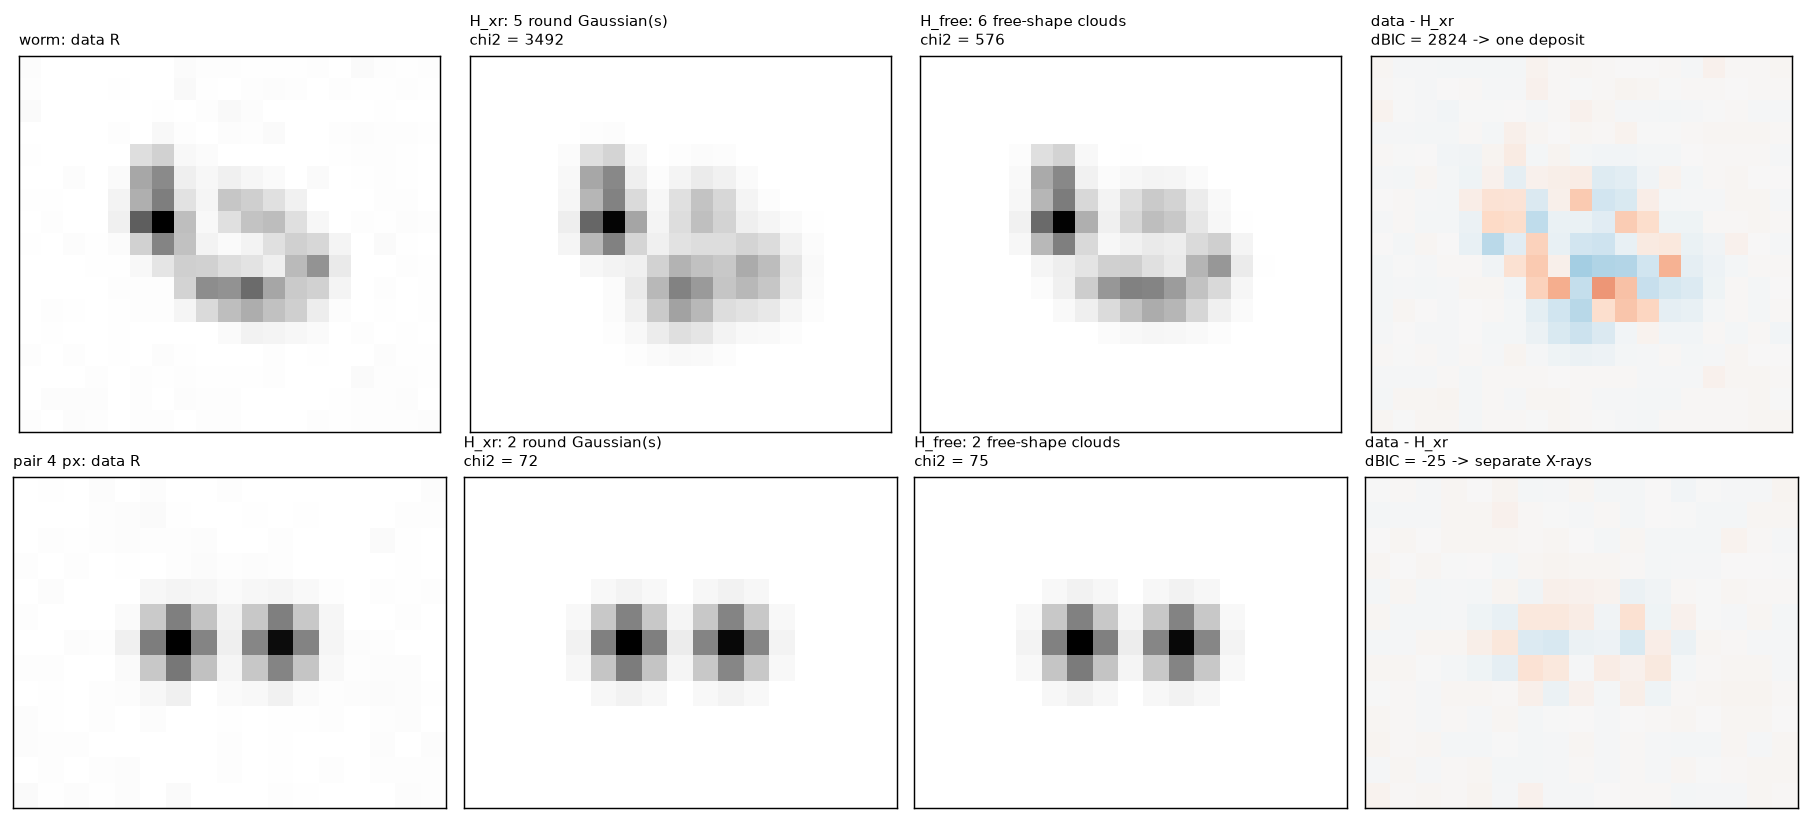
\includegraphics[width=\textwidth]{figures_current/fig13_island_example.png}
\caption{The island test on two islands of the test image. Top, the worm: 5 round Gaussians cannot follow the bent track
($\chi^2$ 3492, structured residual); 6 free-shape clouds can ($\chi^2$ 576); $\Delta\mathrm{BIC}=2824\to$ one deposit. Bottom,
the 4-px pair: both descriptions fit equally well ($\chi^2$ 72 vs 75), the round one has fewer parameters,
$\Delta\mathrm{BIC}=-25\to$ two separate X-rays.}
\end{figure}

\begin{figure}[H]\centering
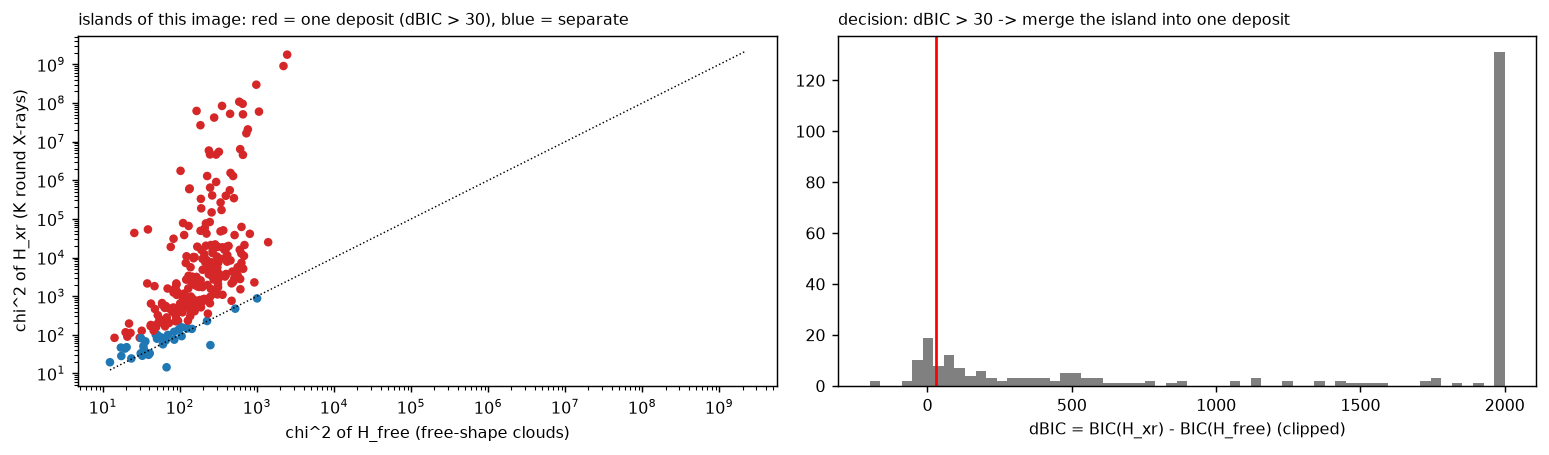
\includegraphics[width=\textwidth]{figures_current/fig09_island_bic.png}
\caption{All islands of the test image: $\chi^2$ of the two hypotheses (left) and $\Delta\mathrm{BIC}$ (right). Red: one
deposit (tracks, worms, irregular blobs); blue: separate X-rays.}
\end{figure}

%======================================================================================================
\section{Step 6 --- energy, shape, purity}\label{sec:energy}

\paragraph{Energy by sharing.} The cluster responsibility of pixel $p$ is $\tilde r_{pc}=\sum_{k\in c}g_k(p)/M_p$ (sum over the
clouds of cluster $c$), and
\begin{equation}
\boxed{\;E_c=\sum_p\tilde r_{pc}\,R_p\;}\qquad[\el;\ \times3.74\ \mathrm{eV/\el}\ \text{for keV}]
\end{equation}
The \textbf{measured} charge $R_p$ is shared (not the model), so the energy does not depend on the Gaussian being exact; shared
pixels are split, never counted twice.
\begin{itemize}
\item \textbf{Satellites.} A cluster with $E<1\,\%$ of a neighbour's energy \emph{and} $E<1$\,keV whose centre lies in that
neighbour's domain or within $6\sigma$ (Mahalanobis) of one of its clouds (within 20\,px) is a tail fragment and is merged into
it. Real X-rays ($>1$\,keV) next to a very large deposit stay their own clusters.
\item \textbf{Growth.} Pixels above the Poisson-tail threshold ($\alpha=0.01$) within 3\,px of a covered pixel and connected to it,
but covered by no cloud (CTI trails along the readout), are added to the nearest cluster.
\end{itemize}

\paragraph{Width.} $\sigma_{xy}^2=\tfrac12(\mathrm{var}_y+\mathrm{var}_x)-\tfrac1{12}$, the second moments of the cluster's shared
charge (unbiased to $\sim$1\,\% for Fe-55 at $\sigma\ge0.4$\,px). Below that the moment is dominated by the noise and dark charge
of the footprint, so a cluster made of one cloud whose EM width is below 0.4\,px reports the EM width instead:

\begin{table}[H]\centering\footnotesize
\begin{tabular}{lcccccc}
\toprule
true $\sigma$ [px] (single 5.9-keV X-rays, 0.15\,\el{} noise) & 0.2 & 0.3 & 0.4 & 0.6 & 1.0 & 1.5 \\
\midrule
reported $\sigma_{xy}$ & 0.250 & 0.304 & 0.401 & 0.600 & 0.997 & 1.505 \\
$E_\mathrm{rec}/E_\mathrm{true}$ & 1.000 & 1.000 & 1.000 & 1.000 & 1.000 & 1.000 \\
\bottomrule
\end{tabular}
\end{table}
\noindent A 0.2-px cloud puts 99\,\% of its charge in one pixel when centred, so its width is barely measurable; either way it
is far below the front/back cut at 1\,px.

\paragraph{Significance.} $E_c\big/\sqrt{\sum_p\tilde r_{pc}^2V_p}$.

\paragraph{Quality flags} (they never change the energy; section~\ref{sec:flags} shows what they do):
\begin{itemize}\itemsep1pt
\item \textbf{blend} --- how much of \emph{other} clusters' predicted charge lies under this cluster's profile, relative to its own:
\begin{equation}
\mathrm{blend}_c=\frac{\sum_p M_p^{(c)}M_p^{(\neg c)}}{\sum_p\big(M_p^{(c)}\big)^2},\qquad
M_p^{(c)}=\tilde r_{pc}M_p,\quad M_p^{(\neg c)}=M_p-M_p^{(c)} .
\end{equation}
0 = isolated; 0.1 = 10\,\% of its profile is shared with neighbours (SExtractor's deblending flag, but as a number);
\item \textbf{ped} --- the local pedestal: the 25th percentile of $R$ in a ring 5--8\,px around the centre (a charge sheet under
the cluster);
\item \textbf{peakfrac} --- the share of the cluster's fitted charge in its largest cloud (merged neighbours give $<1$);
\item \textbf{$\chi^2$} --- $\frac{1}{n_c}\sum_{p:\tilde r_{pc}>0.5}(R_p-M_p)^2/(V_p+M_p)$, the fit quality of its own model;
\item \textbf{edge} --- touches the 2-px border of the active area; \textbf{saturated} --- a pixel at an ADC-limit plateau (the
energy is then a lower limit).
\end{itemize}

\begin{figure}[H]\centering
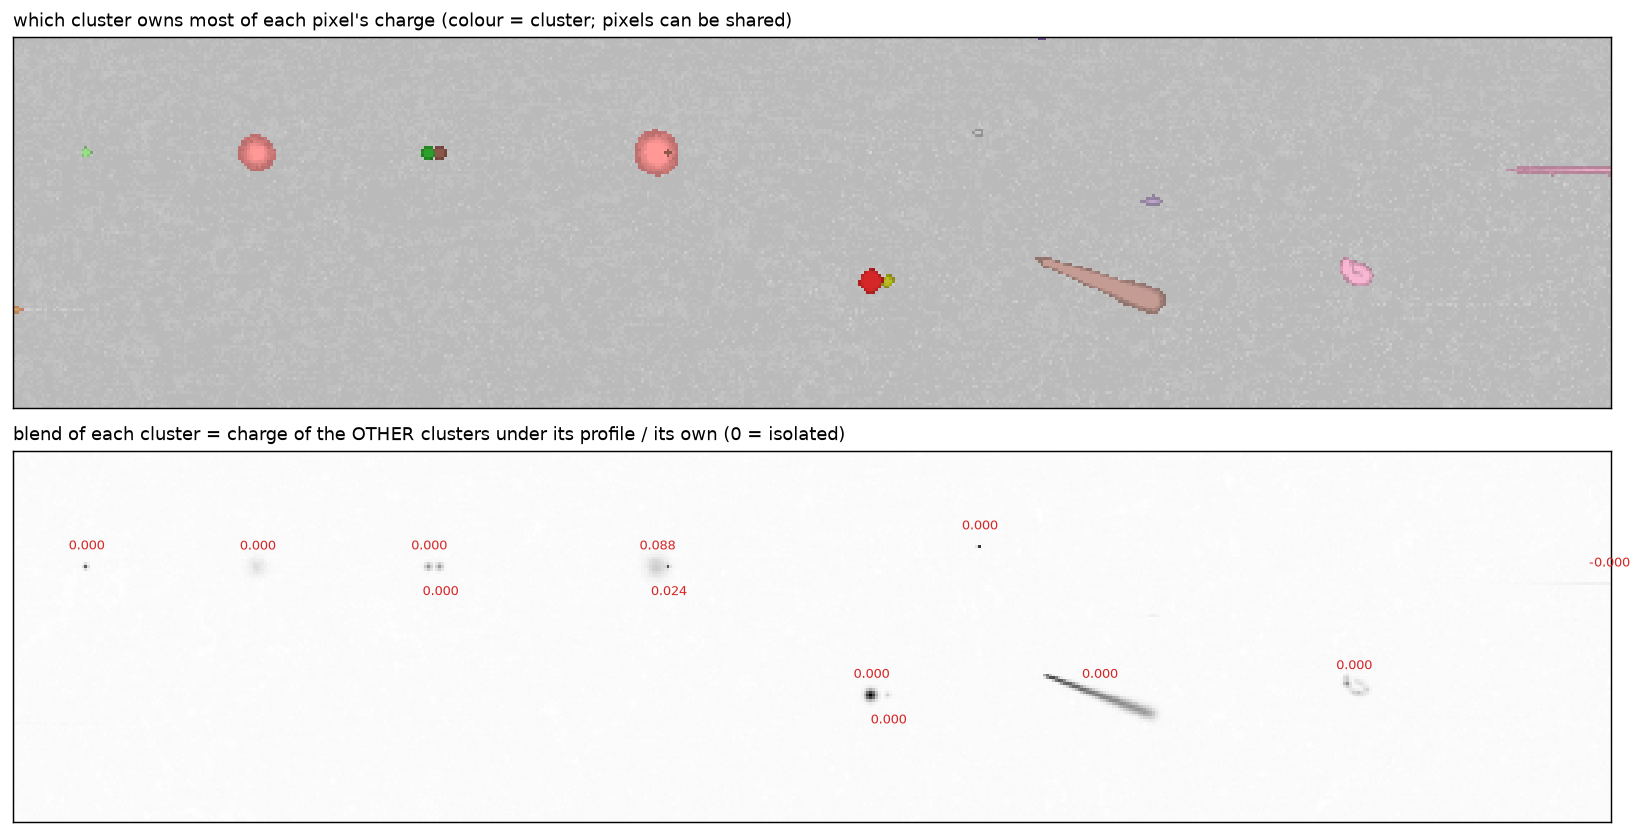
\includegraphics[width=\textwidth]{figures_current/fig10_ownership_blend.png}
\caption{Top: which cluster owns most of each pixel's charge. Bottom: blend of each cluster (0 for isolated clusters; 0.088 /
0.024 for the sharp X-ray on the diffuse one, whose profiles overlap).}
\end{figure}

%======================================================================================================
\section{Step 7 --- few-electron events}

On electron-counting CCDs (median $s<0.35$\,\el, where rounding to whole electrons is reliable) three extra rules apply.

\paragraph{Detection dark charge.} The fitted $\lambda$ map fluctuates far below and above the truth where it is tiny (a fit cell
holds only a few dark electrons). For every few-electron test the dark charge is therefore at least the one implied by the
measured rate of \emph{isolated} single-electron pixels (no other counted pixel within 2\,px; real events come with neighbours),
smoothed over $\pm30$ rows, with the rounding miscounts of the read noise included, plus the hot-column excess.

\paragraph{Counting energies.} For clusters below 100\,\el, the analog sum adds the read noise of every pixel ($\sqrt N\,s$,
0.5\,\el{} for 13 pixels at 0.15\,\el), so the charge is often off by one. Instead each pixel the cluster mostly owns
($\tilde r>0.5$) is \textbf{rounded} to whole electrons and the expected dark charge is subtracted:
\begin{equation}
E_c^\mathrm{count}=\sum_{p:\ \tilde r_{pc}>0.5}\Big(\mathrm{round}(Q_p-o_p)-\lambda_p\Big).
\end{equation}

\paragraph{Counting finder.} An 8-connected group of at most 9 pixels with $\mathrm{round}(Q_p-o_p)\ge1$, not covered by any
cluster, is scored by the probability of its observed counts under dark charge and read noise alone, with a trial factor for
its shape:
\begin{equation}
T=-\sum_{i\in g}\ln P(n_i\,|\,\lambda_i,s_i)-\ln N_\mathrm{shapes}(m),\qquad
P(n\,|\,\lambda,s)=\sum_k \mathrm{Pois}(k;\lambda)\Big[\Phi\big(\tfrac{n+\frac12-k}{s}\big)-\Phi\big(\tfrac{n-\frac12-k}{s}\big)\Big],
\end{equation}
with $N_\mathrm{shapes}(m)$ the number of 8-connected shapes of $m$ pixels. The group is kept as a ``low-E'' event when $T$
exceeds the value exceeded by 0.08 groups per Mpix in 10--50 blank images simulated from the image's own background
(fixed seed); the analytic bound $\ln(N_\mathrm{pix}/F)$ is used only when the blanks have too few groups.

\begin{figure}[H]\centering
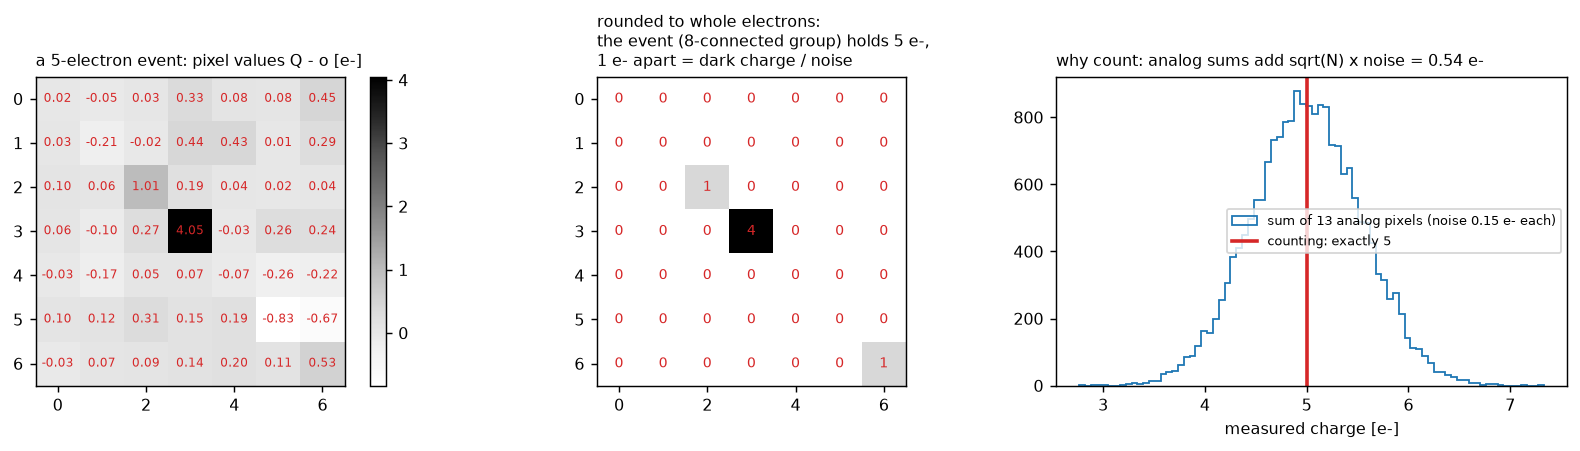
\includegraphics[width=\textwidth]{figures_current/fig11_counting.png}
\caption{A 5-electron event: analog pixel values, the same rounded to whole electrons (the event's 8-connected group holds
5\,\el; the 1\,\el{} in the corner is a separate dark-charge or noise pixel), and why counting is exact while an analog sum over
13 pixels spreads by $\pm0.5$\,\el.}
\end{figure}

%======================================================================================================
\section{Step 8 --- classes}

Every cluster gets a label from its shape: \textbf{low-E} ($E<0.5$\,keV); \textbf{x-ray} / \textbf{x-ray diffuse} (one round
cloud or extent $<6$\,px; diffuse if $\sigma_{xy}\ge1$\,px); \textbf{alpha} ($>1$\,MeV); \textbf{artifact-row / -column} (thin,
straight and aligned with a row or column: serial-register streaks, hot columns); \textbf{muon} (long, straight skeleton: length
$\ge10$\,px, scatter of the cloud centres about a line $<1$\,px and $<6\,\%$ of the length, \emph{and} at least 2.5\,keV per
projected pixel --- a minimum-ionising particle deposits $\sim$4\,keV per 15-\textmu m pixel; a straight track below that is
``extended''); \textbf{worm} (everything else extended). Labels are only checked on injected objects (alpha 0.94--1.00, x-ray
0.8, muon/worm swap $\sim$30\,\%).

%======================================================================================================
\section{After \AGMX: the few-electron candidate catalogue}\label{sec:fecand}

A per-event decision at a fixed fake rate cannot do what a rare-event search needs at the lowest dark currents (a 2-\el{}
single pixel from dark charge is indistinguishable from a real one). For electron-counting images (read noise $<0.35$\,\el)
\code{run\_AGMX} and \code{run\_WADERs --clusterer agmx} therefore also write
\code{fe\_candidates/<image>\_ext<n>\_fe\_candidates.csv} and \code{.json} (\code{clustering\_tests/fe\_candidates.py}), in the
style of the low-background experiments (DAMIC-M, SENSEI):
\begin{itemize}
\item \textbf{candidates}: every group of touching pixels with 2--20 counted electrons ($\le9$ pixels): position, charge,
pixels, local dark charge and read noise, the statistic $T$, $n_\mathrm{exp}$ = the expected number of dark-charge groups per
image at least as unlikely in the clean area (simulated blanks of the image's own occupancy-based dark charge; analytic tail
beyond them) and $p_\mathrm{image}=1-e^{-n_\mathrm{exp}}$;
\item \textbf{mask flags} (nothing is removed): halo within $5\sqrt{E/\mathrm{keV}}$\,px (5--60\,px) of an \AGMX{} cluster,
charge-transfer trails along its row and column ($E>1$\,keV, 50\,px), hot columns, the edge (5\,px), overlap with an \AGMX{}
cluster; \code{clean} = no flag;
\item \textbf{summary}: the isolated single-electron rate, the clean area, and per class (charge, pixels) the observed clean
candidates and the number expected from dark charge alone.
\end{itemize}

\begin{table}[H]\centering\small
\begin{tabular}{lccc}
\toprule
dark charge [\el/pix] & 2\,\el{} in 1\,px & 2\,\el{} in 2\,px & 3\,\el{} in 3\,px \\
\midrule
0.0005 & 5 / 5.2 & 58 / 48.2 & 0 / 0.1 \\
0.001 & 14 / 12.7 & 120 / 114.8 & 0 / 0.7 \\
0.003 & 89 / 93.4 & 731 / 734.0 & 11 / 13.4 \\
\bottomrule
\end{tabular}
\caption*{Observed / expected clean candidates in 10 simulated blank images (1.7\,Mpix each). Injected 3-\el{} events are
listed in 99\,\% of cases (median $n_\mathrm{exp}=0.008$ per image). The blanks are generated from the same pixel model the
catalogue assumes, so this checks the bookkeeping, not real-detector backgrounds.}
\end{table}

%======================================================================================================
\section{The worked example}

The test scene of figure~\ref{fig:overview}: truth versus both methods (energies in keV).

\begin{table}[H]\centering\small
\begin{adjustbox}{max width=\linewidth}
\begin{tabular}{llll}
\toprule
deposit & truth & \AGMX & WADERs \\
\midrule
sharp Fe-55 & 6.06 & 6.05 x-ray & 6.06 \\
diffuse Fe-55 ($\sigma$ 1.6\,px) & 5.81 & 5.81 x-ray diffuse & 5.82 \\
pair, 4\,px apart & 6.20 + 5.77 & \textbf{6.19 + 5.78} & 11.98 (merged) \\
diffuse 17.75\,keV + sharp Fe-55 3\,px away & 18.07 + 5.82 & \textbf{18.13 + 5.78} (sum conserved) & 23.97 (merged) \\
59.5\,keV + faint 1.5\,keV 6\,px away & 59.32 + 1.37 & 59.31 + 1.36 & 59.35 + 1.36 \\
muon (40\,px, minimum ionising) & 228.62 & 228.61 muon & 228.79 \\
worm & 16.20 & 16.19 worm & 16.24 \\
5-electron event & 0.019 & not found & 0.015 \\
\bottomrule
\end{tabular}
\end{adjustbox}
\end{table}

The 5-\el{} event (4\,\el{} in one pixel) sits at $\sim$0.07\,\el/pix dark charge: a group this size is not significant at
\AGMX's calibrated fake rate of 0.08 per Mpix there, while WADERs' 30$\sigma$ seed (3.6\,\el) catches it but has no
fake-rate control (section~\ref{sec:lowe}).

%======================================================================================================
\section{Performance}\label{sec:perf}

All tests use the same injected objects for every method (same random seeds), plus real lines. The code version of each
test is given in its heading.

\subsection{The crowded CCD: Am-241 10--30\,keV constrained fit (code of 27 October)}
29 images, EXT4 (in one corner every pixel holds $>20$\,\el), Np L lines with fixed intensity ratios (L\'epy et al.\ 2008), one
energy scale $k$; $Z$ = combined significance of the Np L lines and $\gamma$\,26.3.

\begin{table}[H]\centering\small
\begin{adjustbox}{max width=\linewidth}
\begin{tabular}{lcccccccc}
\toprule
clustering (cut) & clusters & $k$ & dev/ndf & Np L$\alpha$ & L$\beta$ & L$\gamma$ & $\gamma$\,26.3 & Ag K \\
\midrule
WADERs ($\sigma_{xy}<0.7$) & 62\,665 & 0.9840 & 1.74 & 4.0 & 15.5 & 16.0 & 14.8 & 12.9 \\
\textbf{\AGMX{} ($\sigma_{xy}<0.7$, blend $<0.02$)} & 73\,350 & \textbf{1.0006} & 2.59 & 5.0 & \textbf{22.4} & \textbf{20.6} & \textbf{21.1} & \textbf{18.3} \\
\AGMX{} (+ ped $<10$) & 45\,464 & 0.9990 & 2.12 & 3.6 & 17.4 & 15.9 & 18.0 & 15.6 \\
\bottomrule
\end{tabular}
\end{adjustbox}
\end{table}
\noindent Combined $Z$: WADERs 27.1, \AGMX{} 37.4 (29.9 with the pedestal cut). The lines are higher above the continuum and at
the right energy. Not understood: the deviance per degree of freedom is higher than WADERs' (2.59 vs 1.74), i.e.\ the spectrum
between the lines is described less well; it rose when the exact pixel model was introduced (1.75 before, on the same images).
$\sigma_{xy}$ is a different width estimate from panaSKImg's, so the 0.7 cut is not the same selection for both.

\begin{figure}[H]\centering
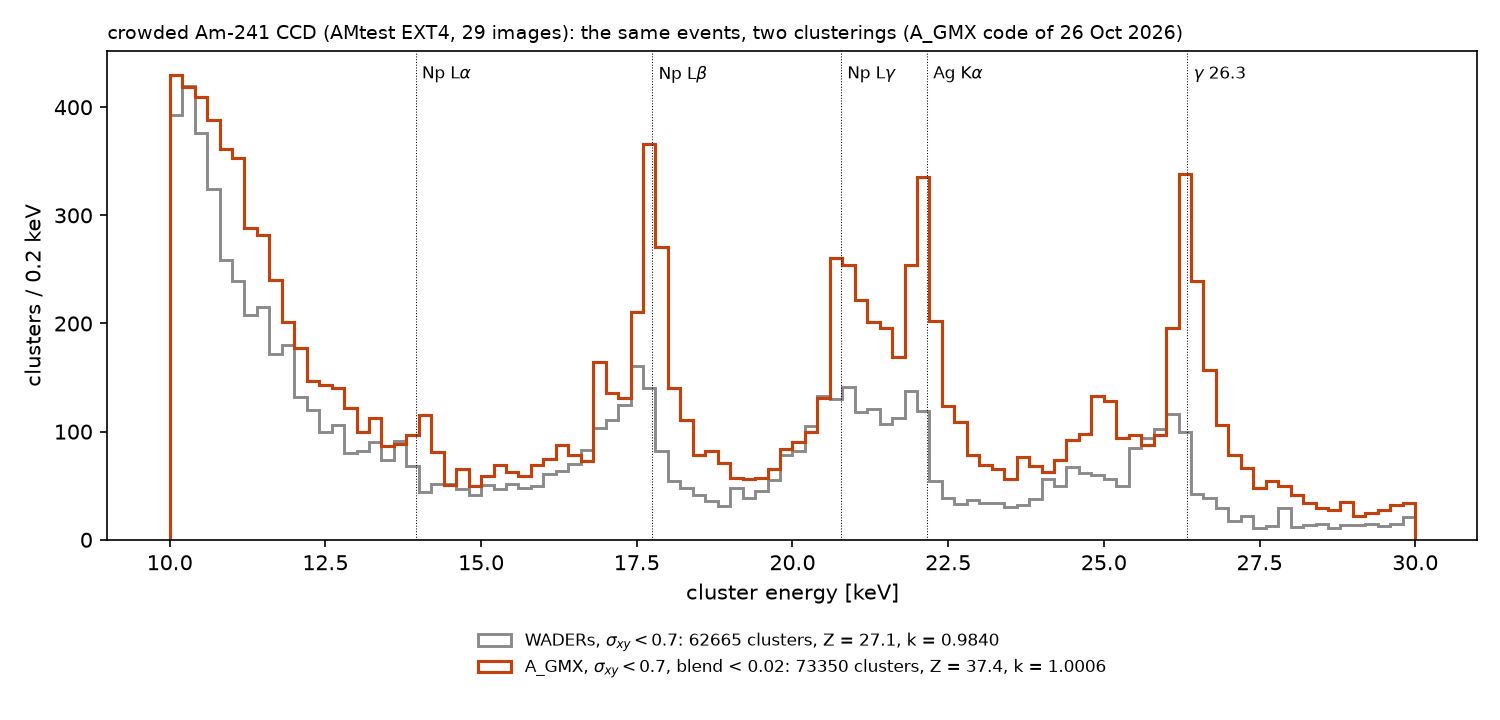
\includegraphics[width=0.95\textwidth]{figures/figC1_crowded_current.png}
\caption{The 10--30-keV spectra of the crowded CCD, WADERs vs \AGMX{} (blend $<0.02$): the same events, the lines about twice as
high above the continuum.}\label{fig:crowded}
\end{figure}

\subsection{Fe-55 front and back side through the full pipeline (code of 27 October)}
DM25 and DM09 (ACM 109), Image\_5, 3 images $\times$ 4 CCDs each, the full \code{run\_WADERs} chain with the $g(n)$ gain
correction, composite-macro definitions (4.5--7\,keV; front $\sigma_{xy}<1$\,px, back $>1$):
\begin{table}[H]\centering\small
\begin{tabular}{lccc}
\toprule
 & WADERs nominal & WADERs + $g(n)$ & \AGMX{} + $g(n)$ \\
\midrule
DM25 (EXT2--4): K$\alpha$ back $-$ front & $-1.0\,\%$ & $-2.9\,\%$ & $\mathbf{-0.06\,\%}$ \\
DM25: back-side K$\alpha$ width & 112\,eV & 138\,eV & \textbf{70\,eV} \\
DM25: back-side rms of the composite profile 3--4\,px from the centre & 1.10--1.37\,px & 1.10--1.37\,px & 1.42--1.58\,px \\
DM09 (EXT1,3,4): K$\alpha$ back $-$ front & $+1.6\,\%$ & $+0.1\,\%$ & $\mathbf{-0.09\,\%}$ \\
DM09, noisy image (noise 0.30\,\el): back side & & $-5$ to $-6.5\,\%$ & $\mathbf{-0.2\,\%}$ \\
\bottomrule
\end{tabular}
\end{table}
\noindent WADERs' back-side loss is charge cut by its thresholds, which scale with the image noise (no loss on DM09's quiet
images, 5--6.5\,\% on its noisy one, $\sim$3\,\% on DM25). Nominal WADERs looks better on DM25 only because two errors cancel:
panaSKImg's single gain is below the low-charge gain there, so the low-charge pixels of back-side clusters read $\sim$3\,\% high.
The widths in the \AGMX{} files include low-charge noise pixels of the footprint; the energies are the cleaner evidence.

\subsection{Sharp X-rays next to diffuse ones (simulation, code of 27 October)}
Skipper blanks (0.1\,\el/pix, 0.16\,\el{} noise), 5.9-keV X-rays, 777 scenes of each kind:
\begin{table}[H]\centering\footnotesize
\begin{tabular}{llcc}
\toprule
scene & cluster & found & $|E/E_\mathrm{true}-1|<5\,\%$ \\
\midrule
isolated sharp ($\sigma$ 0.15--0.35) & sharp & 1.000 & 1.000 \\
sharp 3\,px from diffuse ($\sigma$ 1.2--1.6) & sharp / diffuse & 0.988 / 0.981 & 0.967 / 0.967 \\
two sharp 3\,px apart & sharp & 0.940 & 0.862 \\
isolated diffuse ($\sigma$ 1.0--1.6) & diffuse & 1.000 & 1.000 \\
\bottomrule
\end{tabular}
\end{table}
\noindent With a Gaussian evaluated at the pixel centre instead of the exact pixel integral, the sharp-on-diffuse case was found
in 0.78 and within 5\,\% in only 0.35 of the scenes.

\subsection{Few-electron events at low dark current (code of 26--27 October)}\label{sec:lowe}
Simulated images (0.15\,\el{} read noise), 1800 events of 2--5\,\el{} (Gaussian $\sigma$ 0.2--0.6\,px), 30 blank images per dark
charge; full \AGMX:
\begin{table}[H]\centering\small
\begin{tabular}{lccc}
\toprule
dark charge [\el/pix] & 3\,\el{} found & 4\,\el{} found & fakes per 1.7\,Mpix \\
\midrule
0.0001 & 0.96 & 1.00 & 0.30 \\
0.0005 & 0.93 & 0.99 & 0.37 \\
0.001 & 0.85 & 1.00 & 0.07 \\
0.003 & 0.40 & 0.96 & 0.07 \\
0.01 & 0.04 & 0.53 & 0.23 \\
\bottomrule
\end{tabular}
\end{table}
\noindent The remaining fakes at the lowest dark currents are mostly single pixels with 2\,\el{} (about 0.5 per image at
$5\times10^{-4}$\,\el/pix from dark charge and rounding miscounts), indistinguishable from a real 2-\el{} event: that is what the
candidate catalogue (section~\ref{sec:fecand}) is for. WADERs needs $\gtrsim10$\,\el{} at low dark charge.

\begin{figure}[H]\centering
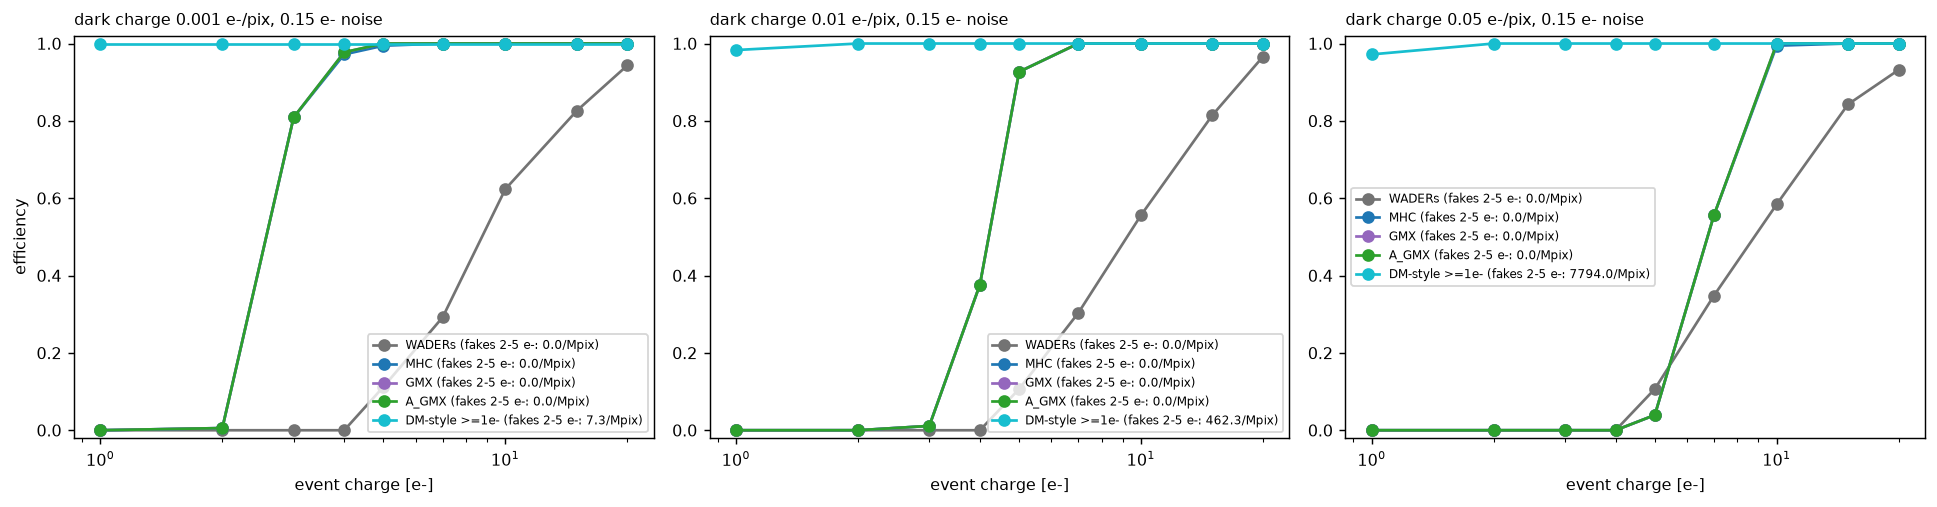
\includegraphics[width=\textwidth]{figures/fig24_few_electron.png}
\caption{Efficiency against event charge at three dark charges (code of 25 October, before the detection dark charge and the
calibrated threshold; the table above is the current code).}
\end{figure}

\subsection{Real data: Fe-55 and Am-241 injections and K$\alpha$ (code of 27 October)}
A subset of the wide test (every 12th Fe-55 image-CCD, every 6th Am-241; 80 image-CCDs), the current pixel model against the
Gaussian-at-centre model: Fe-55 injected pairs 4\,px apart resolved 0.907 $\to$ 0.941, Am-241 0.607 $\to$ 0.655; real front-side
K$\alpha$ changed by $-0.2$\,eV (median over image-CCDs); the $\chi^2$ flag of K$\alpha$ clusters median 6.46 $\to$ 1.31.

\subsection{The wide test: every image on the machine (code of 25 October)}
878 image-CCDs from 16 data sets (Fe-55 production modules DM01--DM28 and PD06--08; Am-241 AMTEst and PD06/DM12; the skip-noise
study). Per image-CCD: 12 Fe-55 clusters ($\sigma$ 0.3--1.6\,px), 4 muons, 4 worms, 4 pairs 4\,px apart. Success = one cluster
with energy within 5\,\% (pairs: both, within 10\,\%). ``WADERs'' here is a hysteresis reimplementation with the WADERs
thresholds.

\begin{figure}[H]\centering
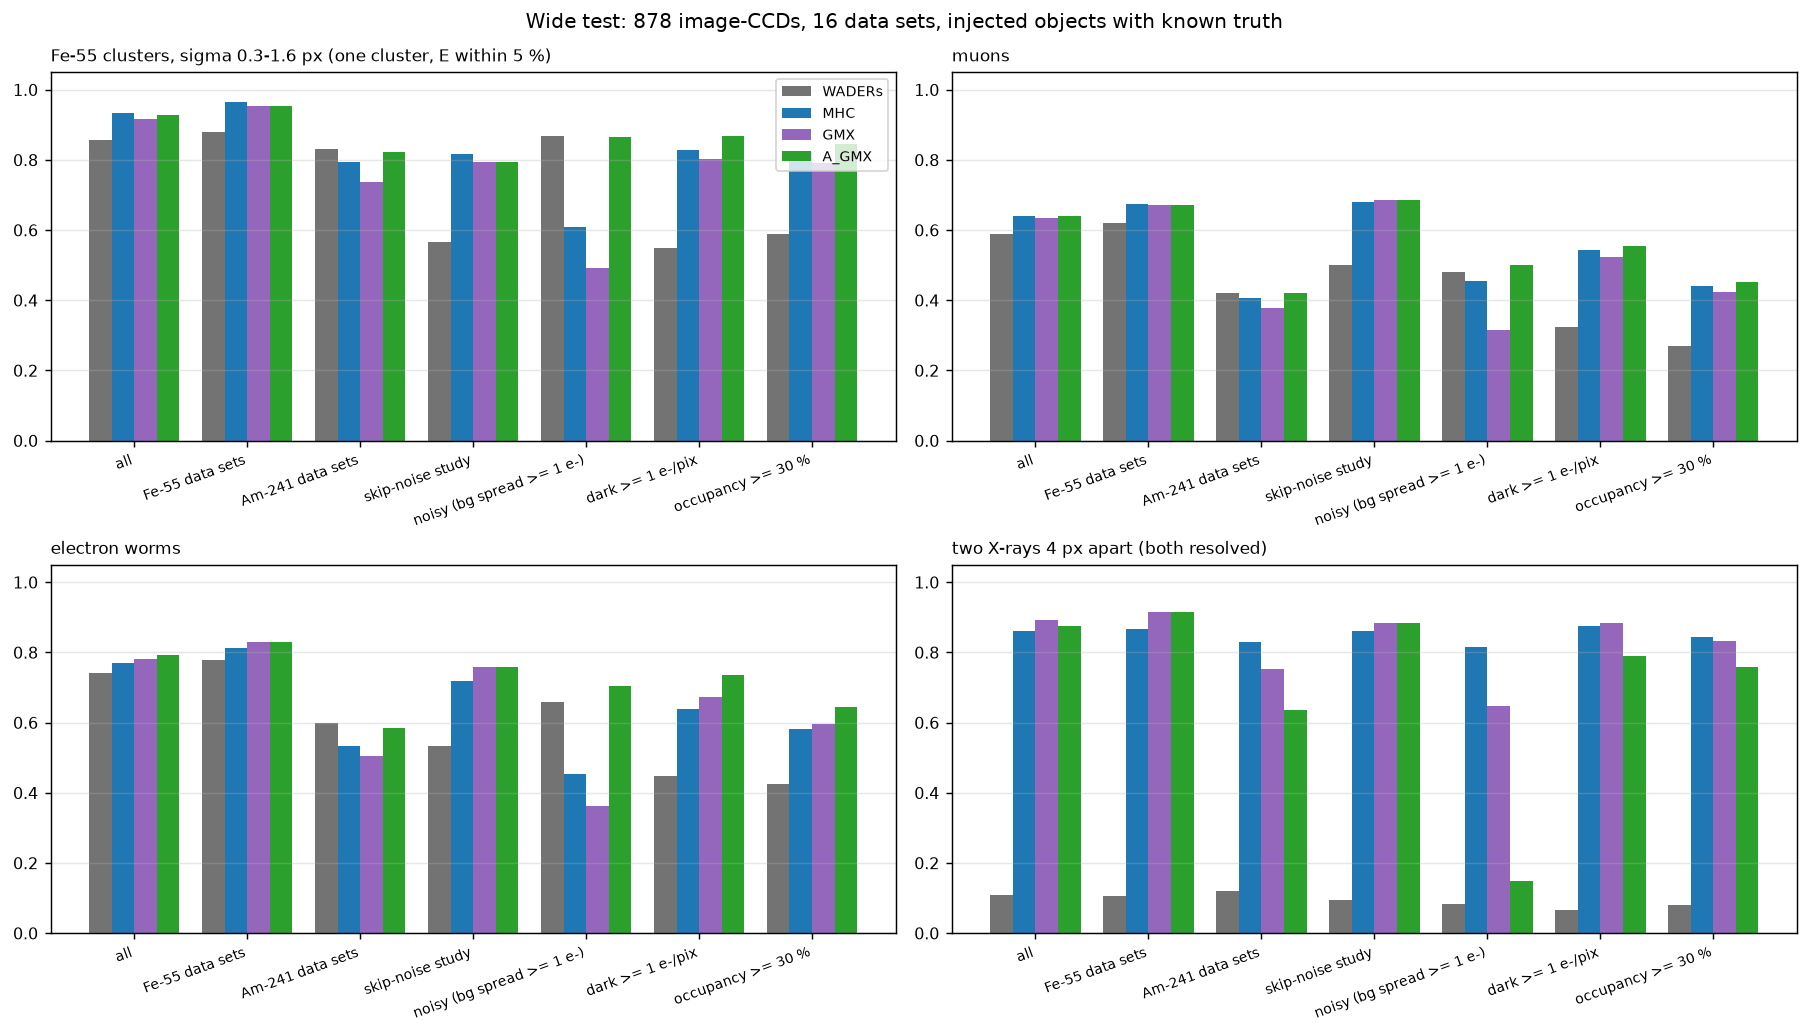
\includegraphics[width=\textwidth]{figures/fig20_wide_vs_waders.png}
\caption{Success fractions by object type and image condition for WADERs, MHC, GMX and \AGMX.}
\end{figure}

%WIDE_TABLE_START
\begin{table}[H]\centering\small
\begin{adjustbox}{max width=\linewidth}
\begin{tabular}{lcccccc}
\toprule
method & Fe-55 ok & Fe-55 $E$ rms & muon & worm & pair 4\,px & s / image-CCD \\
\midrule
WADERs & 0.856 & 0.52\,\% & 0.59 & 0.74 & 0.11 & 0.01 \\
B auto & 0.905 & 0.59\,\% & 0.62 & 0.78 & 0.13 & 0.01 \\
MFD+G & 0.933 & 0.21\,\% & 0.18 & 0.37 & 0.94 & 0.14 \\
hybrid v1 & 0.873 & 0.20\,\% & 0.58 & 0.66 & 0.84 & 0.02 \\
hybrid v2 & 0.930 & 0.21\,\% & 0.63 & 0.68 & 0.85 & 0.05 \\
MHC & 0.933 & 0.21\,\% & 0.64 & 0.77 & 0.86 & 1.61 \\
adaptive (MHC engine) & 0.931 & 0.21\,\% & 0.64 & 0.77 & 0.83 & 1.26 \\
GMX & 0.916 & 0.19\,\% & 0.63 & 0.78 & 0.89 & 0.69 \\
\textbf{\AGMX} & \textbf{0.927} & \textbf{0.19\,\%} & \textbf{0.64} & \textbf{0.79} & \textbf{0.88} & 0.69 \\
\bottomrule
\end{tabular}
\end{adjustbox}
\caption*{Wide test, all 878 image-CCDs.}
\end{table}
%WIDE_TABLE_END

\subsection{Fe-55: energy versus cluster width, pairs, real K$\alpha$ (code of 25 October)}
DM09/DM10 (EXT1, EXT4, images 0--1; 220 injected clusters per width and CCD; pairs of $\sigma$ 1.4-px clusters).

\begin{figure}[H]\centering
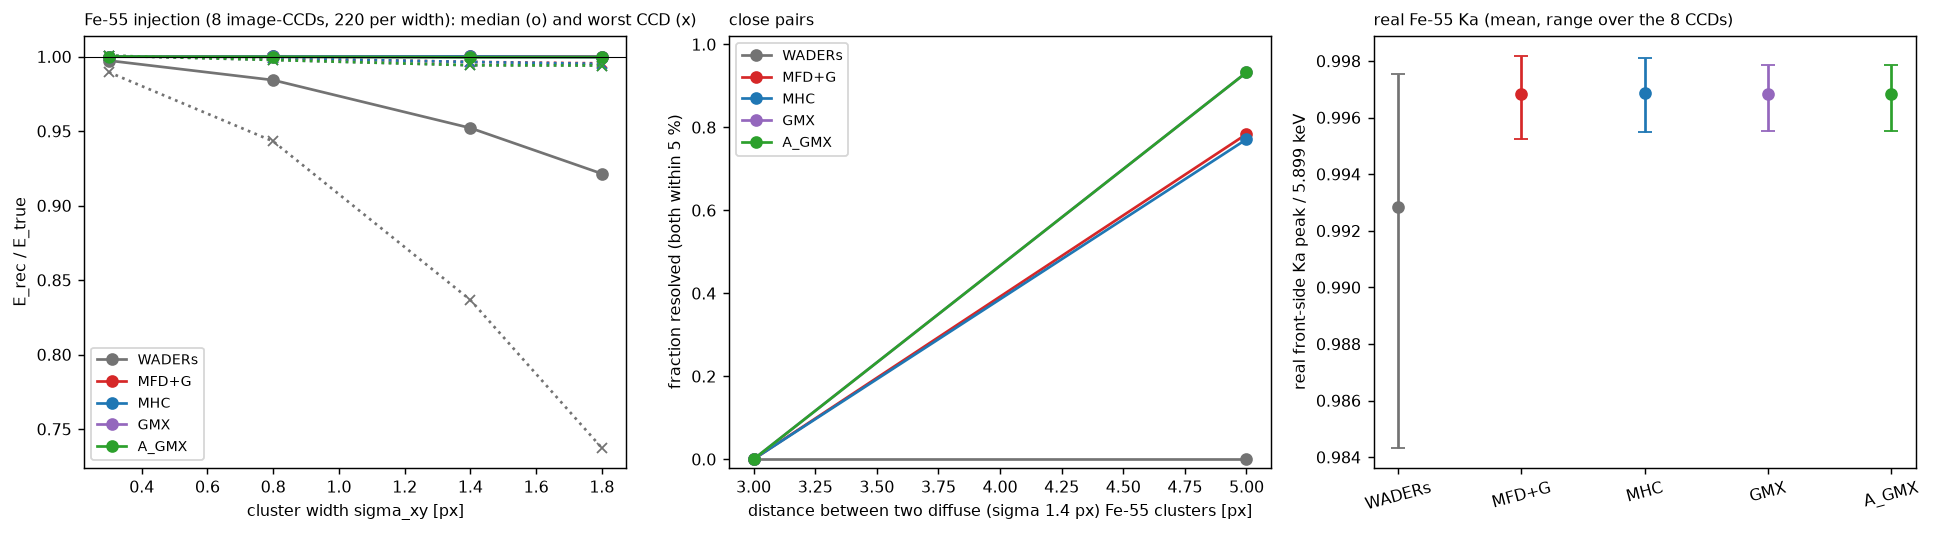
\includegraphics[width=\textwidth]{figures/fig22_fe55.png}
\caption{Left: median (circles) and worst-CCD (crosses) energy ratio against cluster width. Middle: diffuse pairs resolved.
Right: real front-side K$\alpha$ over the 8 CCDs.}\label{fig:fe55}
\end{figure}

\begin{table}[H]\centering\small
\begin{adjustbox}{max width=\linewidth}
\begin{tabular}{lccccccc}
\toprule
method & $\sigma$ 0.3 & 0.8 & 1.4 & 1.8\,px & pair 5\,px & real K$\alpha$/5.899 & spread \\
\midrule
WADERs & 0.9974 (0.990) & 0.9843 (0.943) & 0.9521 (0.837) & 0.9214 (0.737) & 0.00 & 0.9928 & 1.32\,\% \\
MFD+G & 1.0001 (1.000) & 1.0002 (0.999) & 1.0001 (0.996) & 0.9999 (0.995) & 0.78 & 0.9968 & 0.29\,\% \\
MHC & 1.0001 (1.000) & 1.0002 (0.999) & 1.0001 (0.996) & 0.9998 (0.995) & 0.77 & 0.9969 & 0.26\,\% \\
\textbf{\AGMX} & 1.0001 (1.001) & 0.9999 (0.998) & 0.9996 (0.994) & 0.9997 (0.994) & \textbf{0.93} & 0.9969 & \textbf{0.23\,\%} \\
\bottomrule
\end{tabular}
\end{adjustbox}
\caption*{Median $E_\mathrm{rec}/E_\mathrm{true}$ (worst CCD in brackets) per cluster width; pairs resolved; real K$\alpha$.}
\end{table}

\subsection{Injected tracks, alphas and artifacts in real Am-241 images (code of 25 October)}
\begin{figure}[H]\centering
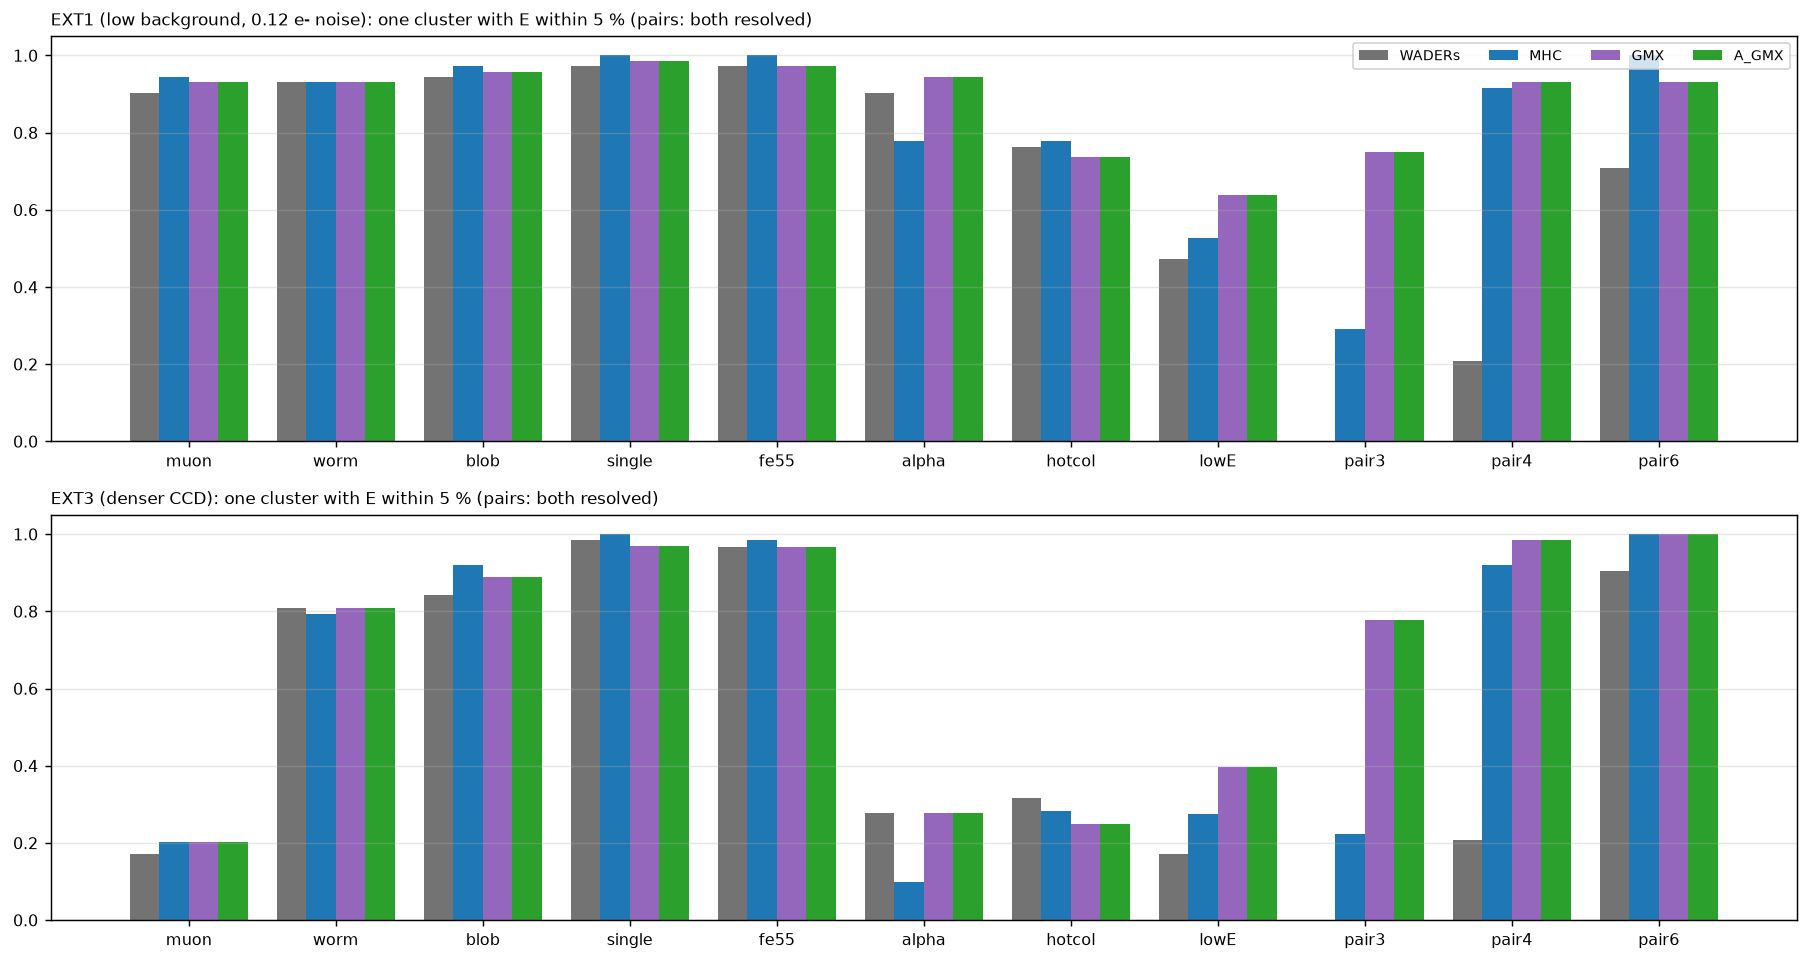
\includegraphics[width=\textwidth]{figures/fig23_tracks.png}
\caption{EXT1 (low background) and EXT3 (denser CCD): success per object type.}
\end{figure}

\begin{table}[H]\centering\footnotesize
\begin{adjustbox}{max width=\linewidth}
\begin{tabular}{lccccccccccc}
\toprule
method & muon & worm & blob & single & fe55 & alpha & hotcol & lowE & pair3 & pair4 & pair6 \\
\midrule
WADERs & 0.90 & 0.93 & 0.94 & 0.97 & 0.97 & 0.90 & 0.76 & 0.47 & 0.00 & 0.21 & 0.71 \\
MFD+G & 0.19 & 0.28 & 0.97 & 1.00 & 1.00 & 0.78 & 0.00 & 0.47 & 0.29 & 0.99 & 1.00 \\
MHC & 0.94 & 0.93 & 0.97 & 1.00 & 1.00 & 0.78 & 0.78 & 0.53 & 0.29 & 0.92 & 1.00 \\
\textbf{\AGMX} & 0.93 & 0.93 & 0.96 & 0.99 & 0.97 & \textbf{0.94} & 0.74 & \textbf{0.64} & \textbf{0.75} & 0.93 & 0.93 \\
\bottomrule
\end{tabular}
\end{adjustbox}
\caption*{EXT1, 3 images $\times$ 3 seeds: success fraction per object type. The injected muons were fainter than minimum
ionising (0.94\,keV per pixel); the harness now has physical muons (\code{MUON\_PHYS=1}) for the next run.}
\end{table}

\subsection{Run time}
Median per image-CCD: Fe-55 0.9\,s, Am-241 62\,s (code of 27 October; WADERs 0.01\,s). Crowded and high-dark-charge CCDs take
minutes: many seeds and clouds, and the few-electron tests have far more candidate groups.

\begin{figure}[H]\centering
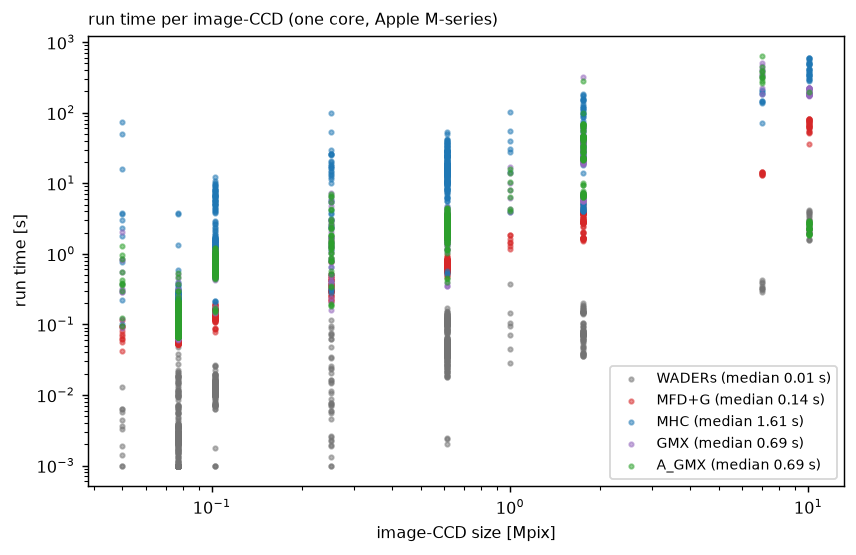
\includegraphics[width=0.7\textwidth]{figures/fig26_runtime.png}
\caption{Run time per image-CCD against its size (code of 25 October; one core, measured with 13 runs in parallel, so times are
indicative).}
\end{figure}

%======================================================================================================
\section{Quality flags and the selection for X-ray lines}\label{sec:flags}

On the crowded Am-241 CCD the 59.5\,keV line has a high-side tail. Injected X-rays (5.9--59.5\,keV) at random positions are
unbiased away from real events (median $E_\mathrm{rec}/E_\mathrm{true}=0.9998$, spread 0.03\,\% at 59.5\,keV); next to real events
every method, WADERs included, adds charge of the neighbour. Two mechanisms, both real charge of other deposits:
\begin{enumerate}
\item \textbf{a charge sheet under the cluster} (dominant on the crowded CCD): many small overlapping deposits make a diffuse
sheet of 20--200\,\el/pix; sharing gives the part under a cluster's footprint to the cluster, which still looks clean. The median
charge in a ring 5--8\,px around 59.5-keV-like clusters is 24\,\el/pix at the peak but 116--218\,\el/pix at 60.5--66\,keV;
\item \textbf{a neighbouring deposit merged into the cluster}: such clusters have several clouds and a bad fit of their own model.
\end{enumerate}
Re-measuring the energy (clipping, local backgrounds, core apertures, a local pedestal subtracted over the footprint) either
changes nothing or adds so much noise that the lines broaden. Energies are therefore left unchanged and the flags of step~6
select clean clusters.

\begin{figure}[H]\centering
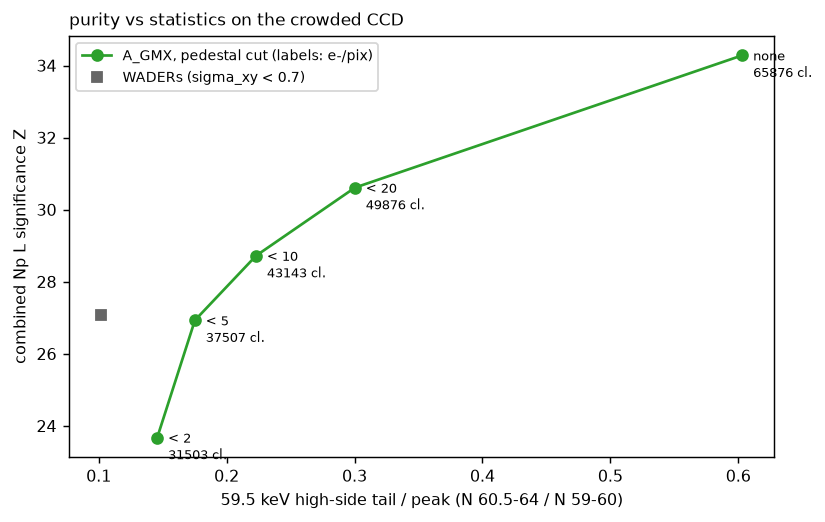
\includegraphics[width=0.7\textwidth]{figures/fig34_pedestal_tradeoff.png}
\caption{Purity against statistics: the 59.5\,keV tail and the Np L significance for pedestal cuts of 20, 10, 5, 2\,\el/pix
(code of 25 October).}\label{fig:tradeoff}
\end{figure}

\paragraph{Recommended selection for spectroscopy.} $\sigma_{xy}<0.7$ (Am-241) or $<1$ (front-side Fe-55), blend $<0.02$,
ped $<10$\,\el/pix, not on the edge; add peakfrac $>0.95$ where merged neighbours matter (crowded fields; not for Fe-55, where it
removes 28--41\,\% of the front-side K$\alpha$ clusters). On Fe-55 images, which have no charge sheet, the ped cut removes at
most 0.1\,\% of the front-side K$\alpha$ clusters. The tables below (code of 25 October) give every Am-241 line fitted alone and
the front-side Fe-55 K$\alpha$ of every data set, with and without the flags.

% generated by clustering_tests/am241_lines_flags.py (contamination_table)
\begin{table}[H]\centering\small
\begin{adjustbox}{max width=\linewidth}
\begin{tabular}{lcccccc}
\toprule
selection (crowded CCD, 29 images) & clusters & 59.5 tail/peak & $k$ & dev/ndf & $Z$ & L$\beta$ / L$\gamma$ / $\gamma$26.3 / Ag K \\
\midrule
WADERs ($\sigma_{xy}<0.7$) & 62\,665 & 0.10 & 0.9840 & 1.74 & 27.1 & 15.5 / 16.0 / 14.8 / 12.9 \\
\AGMX{} ($\sigma_{xy}<0.7$, blend $<0.02$) & 82\,073 & 0.62 & 1.0016 & 1.93 & 34.8 & 20.8 / 19.2 / 19.9 / 18.1 \\
\quad + ped $<10$\,\el/pix & 48\,839 & 0.23 & 0.9994 & 1.55 & 28.7 & 16.2 / 16.0 / 17.3 / 15.3 \\
\quad + ped $<5$\,\el/pix & 41\,344 & 0.18 & 0.9993 & 1.49 & 26.8 & 14.6 / 15.3 / 16.3 / 14.3 \\
\bottomrule
\end{tabular}
\end{adjustbox}
\end{table}
   % generated by clustering_tests/am241_lines_flags.py fit
\IfFileExists{lines_flags_table.tex}{% generated by clustering_tests/am241_lines_flags.py
\begin{table}[H]\centering\scriptsize
\begin{adjustbox}{max width=\linewidth}
\begin{tabular}{llcccccccc}
\toprule
CCD & selection & clusters & Np La & Np Lb & Np Lg & $\gamma$ 26.3 & $\gamma$ 59.5 & 59.5 tail & $k$ (EXT4) \\
\midrule
EXT1 & old A-GMX (sxy$<$0.7, blend$<$0.02) & 13632 & -- & -- & -- & -- & 0.9867 (206) & 0.23 &  \\
EXT1 & new A-GMX (sxy$<$0.7, blend$<$0.02) & 13715 & -- & -- & -- & 0.9716 (251) & 0.9867 (206) & 0.23 &  \\
EXT1 & new + ped$<$10 & 13715 & -- & -- & -- & 0.9716 (251) & 0.9867 (206) & 0.23 &  \\
EXT1 & new + peakfrac$>$0.95 & 13600 & -- & -- & -- & 0.9723 (247) & 0.9867 (208) & 0.23 &  \\
EXT1 & new + ped$<$10 + peakfrac$>$0.95 & 13600 & -- & -- & -- & 0.9723 (247) & 0.9867 (208) & 0.23 &  \\
\midrule
EXT3 & old A-GMX (sxy$<$0.7, blend$<$0.02) & 75580 & -- & 0.9943 (200) & -- & -- & 0.9989 (246) & 0.11 &  \\
EXT3 & new A-GMX (sxy$<$0.7, blend$<$0.02) & 83037 & -- & -- & -- & -- & 0.9989 (246) & 0.11 &  \\
EXT3 & new + ped$<$10 & 81364 & -- & 0.9953 (200) & -- & -- & 0.9988 (242) & 0.10 &  \\
EXT3 & new + peakfrac$>$0.95 & 65083 & -- & 0.9962 (200) & -- & -- & 0.9994 (244) & 0.14 &  \\
EXT3 & new + ped$<$10 + peakfrac$>$0.95 & 63641 & -- & 0.9962 (200) & -- & -- & 0.9994 (239) & 0.13 &  \\
\midrule
EXT4 & old A-GMX (sxy$<$0.7, blend$<$0.02) & 65876 & -- & -- & -- & 1.0038 (273) & 1.0017 (353) & 0.60 & 1.0014 \\
EXT4 & new A-GMX (sxy$<$0.7, blend$<$0.02) & 82073 & -- & -- & -- & 1.0041 (288) & 1.0017 (352) & 0.62 & 1.0016 \\
EXT4 & new + ped$<$10 & 48839 & -- & 0.9977 (200) & -- & 1.0007 (245) & 1.0006 (314) & 0.23 & 0.9994 \\
EXT4 & new + peakfrac$>$0.95 & 70840 & -- & -- & 1.0053 (263) & 1.0046 (296) & 1.0025 (349) & 0.69 & 1.0018 \\
EXT4 & new + ped$<$10 + peakfrac$>$0.95 & 41474 & -- & 0.9983 (200) & -- & 1.0007 (250) & 1.0012 (306) & 0.24 & 0.9993 \\
\bottomrule
\end{tabular}
\end{adjustbox}
\caption*{Every Am-241 line fitted alone: peak / true energy (width in eV); Np L$\beta$ and L$\gamma$ are groups of lines, so their centres are not expected at exactly 17.75 / 20.78\,keV (the constrained fit's $k$ is the check there).}
\end{table}
}{}
\IfFileExists{fe55_flags_tables.tex}{% generated by clustering_tests/summ_wide_flags.py
\begin{table}[H]\centering\footnotesize
\begin{adjustbox}{max width=\linewidth}
\begin{tabular}{lccccccccc}
\toprule
data set & n & Ka old (all) & Ka new (all) & front & front+ped & front+pf & front+both & front lost to ped & front lost to both \\
\midrule
2025-08-27-DM07 DM09 DM10 & 102 & 5.8004 & 5.8000 & 5.7705 (63) & 5.7705 (63) & 5.7772 (62) & 5.7772 (62) & 0.0 \% & 28.7 \% \\
2025-08-30-DM11 DM13 DM14 & 102 & 5.7960 & 5.7955 & 5.7732 (68) & 5.7732 (68) & 5.7915 (65) & 5.7915 (65) & 0.0 \% & 40.5 \% \\
2025-09-03-DM15 DM16 DM17 & 102 & 5.7794 & 5.7789 & 5.7525 (67) & 5.7518 (67) & 5.7721 (65) & 5.7721 (65) & 0.1 \% & 37.4 \% \\
2025-09-06-DM18 DM19 DM20 & 102 & 5.7719 & 5.7715 & 5.7387 (70) & 5.7387 (70) & 5.7524 (69) & 5.7524 (69) & 0.0 \% & 33.6 \% \\
2025-09-13-DM24 DM25 DM26 & 90 & 5.9069 & 5.9070 & 5.8875 (65) & 5.8875 (65) & 5.8895 (66) & 5.8895 (66) & 0.0 \% & 38.0 \% \\
\bottomrule
\end{tabular}
\end{adjustbox}
\caption*{Fe-55 K-alpha per data set: median fitted peak over image-CCDs [keV] (median width eV); old vs new A\_GMX without cuts, new front side with the flag cuts. No K-alpha fit in any image-CCD of: 2025-09-07-DM18 DM19 DM20, 2025-09-09-DM21 DM22 DM23, 2025-09-16-DM08 DM11 DM12, 2025-09-19-DM07 DM27 DM28, 2025-10-31-DM04 DM05 DM06, 2025-11-04-DM10 DM24 DM25, 2025-11-08-PD06 PD07 PD08, 2025-11-13-DM01 DM02 DM03.}
\end{table}

\begin{table}[H]\centering\footnotesize
\begin{adjustbox}{max width=\linewidth}
\begin{tabular}{lcccc}
\toprule
selection & image-CCDs & median K-alpha [keV] & spread [eV] & width [eV] \\
\midrule
old A\_GMX, all clusters & 401 & 5.7934 & 66 & 79 \\
new A\_GMX, all clusters & 401 & 5.7947 & 67 & 80 \\
new, front & 381 & 5.7709 & 69 & 67 \\
new, front, ped<10 & 380 & 5.7704 & 69 & 67 \\
new, front, peakfrac>0.95 & 343 & 5.7851 & 73 & 66 \\
new, front, ped<10, peakfrac>0.95 & 343 & 5.7851 & 73 & 66 \\
\bottomrule
\end{tabular}
\end{adjustbox}
\caption*{Fe-55 K-alpha, all Fe-55 image-CCDs: number fitted, median peak, robust spread over image-CCDs, median width. old = A\_GMX before the 25 October changes, new = with them (satellite limit, flags, audit fixes).}
\end{table}

\begin{table}[H]\centering\footnotesize
\begin{adjustbox}{max width=\linewidth}
\begin{tabular}{lccccc}
\toprule
data sets & image-CCDs & Fe-55 & muon & worm & pair 4 px \\
\midrule
Fe-55 & 705 & 0.951 / 0.954 & 0.672 / 0.672 & 0.829 / 0.829 & 0.912 / 0.915 \\
Am-241 & 115 & 0.819 / 0.824 & 0.424 / 0.422 & 0.585 / 0.585 & 0.622 / 0.635 \\
skip-noise & 58 & 0.799 / 0.792 & 0.675 / 0.680 & 0.780 / 0.775 & 0.899 / 0.888 \\
\bottomrule
\end{tabular}
\end{adjustbox}
\caption*{Injection test (same objects): success old / new A\_GMX.}
\end{table}
}{}

%======================================================================================================
\section{Does \AGMX{} supersede the other methods?}\label{sec:supersede}

\textbf{Yes, as the general clusterer.} Against each alternative:

\begin{table}[H]\centering\footnotesize
\begin{tabularx}{\textwidth}{l>{\raggedright\arraybackslash}X>{\raggedright\arraybackslash}X}
\toprule
method & where it is still better than \AGMX & verdict \\
\midrule
MHC & Fe-55 data sets: Fe-55 success 0.964 vs 0.951 (energies equal); hot columns 0.78 vs 0.74 & \textbf{superseded.} \AGMX{} is
better on crowded images, noisy images, high dark charge, worms, alphas, 3-px pairs (0.75 vs 0.29), diffuse 5-px pairs (0.93 vs
0.77) and energy resolution. Keep the code as a cross-check. \\
hybrid v1 / v2, adaptive (MHC engine), GMX alone & nothing significant & \textbf{superseded}. \\
MFD+G & isolated X-rays only: Fe-55 success 0.972 vs 0.951, faster & \textbf{keep for fast Fe-55 gain calibration}. Not for
tracks (muon 0.18). \\
WADERs & noisy ``unmodelled'' images (where \AGMX{} \emph{is} WADERs-like); speed ($\sim$100$\times$); the established pipeline;
the smoothness of the crowded-CCD spectrum between the lines & \textbf{keep as the reference}; it is what \AGMX{} falls back to. \\
\bottomrule
\end{tabularx}
\end{table}

%======================================================================================================
\section{Limits and open items}
\begin{itemize}
\item \textbf{Crowded-CCD fit quality:} deviance/ndf 2.59 vs 1.74 (WADERs); not understood.
\item \textbf{Background on crowded CCDs:} the fitted dark charge on the crowded CCD is 0.157\,\el/pix (0.093 with the background
model of 24 October), which moves the 59.5-keV peak by about $+0.1$\,keV; which value is right is being tested.
\item \textbf{Unmodelled images} fall back to hysteresis: close pairs are then not resolved; the pixel threshold of 4.5\,\el{}
is a stop-gap.
\item \textbf{Very sharp clusters:} widths below $\approx0.25$\,px are hard to measure.
\item \textbf{EM depends on the seeds}; no global optimum is guaranteed. The island test tolerates 5\,\% non-Gaussianity and has
only been checked on injected objects and Fe-55; real Am-241 tracks have not been inspected by eye.
\item \textbf{Labels:} muon/worm swap $\sim$30\,\%; classes only validated on injections.
\item \textbf{Speed:} minutes on crowded and high-dark-charge CCDs.
\item \textbf{Validation:} the wide, Fe-55-width and track tests are from the code of 25 October; injections use Gaussian clouds,
which is \AGMX's own model; the few-electron blanks are generated from the pixel model the finder assumes.
\end{itemize}

%======================================================================================================
\section{Parameters, code, how to run}

\begin{table}[H]\centering\small
\begin{adjustbox}{max width=\linewidth}
\begin{tabular}{llll}
\toprule
parameter & default & where & meaning \\
\midrule
\code{excess\_ratio}, \code{noise\_max} & 3, 1\,\el & adaptive & unmodelled if $s\ge3\sigma_\mathrm{read}$ and $\ge0.5$\,\el, or $\sigma_\mathrm{read}\ge1$\,\el \\
\code{occ\_thr}, \code{box} & 0.3, 31\,px & adaptive & ``crowded'' label (information) \\
\code{scales} & 0.5, 1, 1.5, 2.5\,px & GMX & matched-filter widths \\
\code{nsig} & 5 & GMX & seed significance (+ Poisson check at the same tail) \\
\code{n\_iter} & 30 (+15 residual, +5 pruning) & GMX & EM iterations \\
\code{nsig\_res} & 5 & GMX & residual-pass seeds \\
\code{sig\_min} & 4 & GMX & prune clouds with S/N below \\
\code{r\_merge}, \code{w\_ratio} & 0.5, 1.6 & GMX & ridge ratio, width ratio for merging \\
\code{f\_bridge}, \code{a\_faint} & 0.1, 50\,\el & GMX & fragments link only to their brightest partner \\
\code{link\_alpha}, \code{island\_max}, \code{bic\_margin} & 0.01, 4000\,px, 100 & GMX & island test \\
\code{f\_sat}, \code{sat\_e\_max} & 0.01, 1\,keV & GMX & satellite absorption (only fragments $<1$\,keV) \\
\code{ped\_ring}, \code{ped\_q} & (5, 8)\,px, 25 & GMX & local pedestal flag (ring, percentile) \\
\code{grow} & 3\,px & GMX & CTI-trail growth \\
\code{count\_fakes}, \code{count\_E\_max} & 0.08 per Mpix, 100\,\el & GMX & few-electron finder, counting energies \\
\bottomrule
\end{tabular}
\end{adjustbox}
\end{table}

\paragraph{Switches} (environment): \code{AGMX\_PIX\_EXACT=0} (Gaussian-at-centre model, island margin 30, no fragment rule),
\code{AGMX\_PHYS\_FIXES=0} (the background, hot-column, counting, width and class rules of before 25 October),
\code{AGMX\_NUMBA=0} (numpy EM), \code{AGMX\_FE\_CANDIDATES=0} (no candidate catalogue).

\begin{lstlisting}[language=Python]
import sys; sys.path.insert(0, "comm_scripts/clustering_tests")
import adaptive as AD
clusters = AD.adaptive_cluster(Q_electrons, valid_mask, engine="gmx")
# each cluster: E [keV], y, x, sxy [px], cls, blend, sig, n_comp, edge, ped [e-/pix], peakfrac, chi2, saturated,
#               regime ('sparse' / 'crowded' / 'unmodelled'), occ
good = [c for c in clusters if c.get("blend", 0) < 0.02 and not c.get("edge")
        and not c.get("ped", 0) >= 10          # not sitting on a charge sheet (crowded fields)
        and c.get("peakfrac", 1) > 0.95]       # not merged with a neighbouring deposit (not for Fe-55)
\end{lstlisting}

Test scripts (all in \code{clustering\_tests/}, README there): \code{wide\_test.py} + \code{wide\_run.py adaptive+GMX} (all images),
\code{adaptive\_validate.py} (tracks, few-electron, Fe-55, crowded), \code{make\_agmx\_figures.py}, \code{make\_agmx\_perf.py}.
Unit tests: \code{python -m unittest discover -s tests}.

\subsection{Running \AGMX{} on WADERs data: cluster files in the WADERs format}\label{sec:running}
\begin{lstlisting}
run_WADERs images.txt --gain-correction --clusterer agmx --composite   # A_GMX files, composite on them
run_WADERs images.txt --gain-correction --clusterer both --composite   # also composite_agmx/ next to composite/
run_AGMX WADERs_analysis_<run> [-j 4] [--per-image] [--no-gaincorr] [--no-fe-candidates]   # a finished run
\end{lstlisting}
It runs on the calibrated image panaSKImg saves for every CCD (\code{<image>\_EXT<n>\_waders.fits.bz2}). With the gain
correction, the image is first converted ADU $\to$ \el{} with the same $g(n)$ curves and anchor as \code{root\_gaincorr/}; a CCD
without a reliable curve keeps its fitted gain, as there. The output is \code{root\_agmx/} and \code{root\_agmx\_gaincorr/}: one
\code{panaSKImg\_clustersRec\_<image>\_ext<n>.root} per CCD, written by \code{src/agmx\_root.py}. Every \AGMX{} cluster (its pixels
and the charge it takes from each, which sums to $E$) becomes a pysimdamicm \code{Cluster} object, the ClusterFinder's own
class, so all branches (positions, \code{wSTD}, \code{fSTD}, PCA, track end points, seed, \code{closest\_cls\_*},
\code{Energy\_PS/AVG}, \dots) are computed by panaSKImg's code. \code{info} and \code{process\_config} are copied from the
CCD's panaSKImg file, and the extra branches \code{agmx\_cls}, \code{agmx\_blend}, \code{agmx\_ped}, \code{agmx\_peakfrac},
\code{agmx\_chi2}, \code{agmx\_sig}, \code{agmx\_regime} and a \code{TNamed agmx\_config} are added. MakeComposite and every
other reader of WADERs files read them unchanged. For electron-counting CCDs the candidate catalogue goes to
\code{fe\_candidates/}.

\paragraph{Check.} \code{clustering\_tests/agmx\_root\_check.py} writes the clusters of real panaSKImg files (EXT1, EXT3 and
EXT4 of an Am-241 image: 1652, 7686 and 5452 clusters) through the writer and compares every branch. They are identical except
in numerically degenerate cases, where panaSKImg's own result depends on the last bits of its inputs (Gaussian fits of profiles
1--3 bins wide, the sign of a PCA eigenvector, PCA of 1--2 pixel clusters, \code{closest\_cls\_*} when the nearest cluster lies
in the same row or column). With the default \code{--clusterer waders} the pipeline output is identical to before. A flag value
of $-999$ in the files means ``not computed'' (e.g.\ \code{agmx\_chi2} of a cluster the mixture did not fit); clusters from the
few-electron finder and the hysteresis branch get \code{edge} and \code{ped} like the others, \code{blend} $=0$ and
\code{peakfrac} $=1$.

%======================================================================================================
\appendix
\section{All performance tables}\label{app:tables}
Generated by \code{clustering\_tests/make\_agmx\_perf.py} from the saved results (code of 25 October; same tests as
section~\ref{sec:perf}; all methods; ``ok'' = one cluster with energy within 5\,\%, pairs: both resolved).
% generated by clustering_tests/make_agmx_perf.py
\paragraph{Wide test, all (878 image-CCDs)}
\begin{table}[H]\centering\footnotesize
\begin{adjustbox}{max width=\linewidth}
\begin{tabular}{lcccccc}
\toprule
method & Fe-55 ok & Fe-55 E rms & muon & worm & pair 4 px & s / image-CCD (median) \\
\midrule
WADERs & 0.856 & 0.52 \% & 0.59 & 0.74 & 0.11 & 0.01 \\
B auto & 0.905 & 0.59 \% & 0.62 & 0.78 & 0.13 & 0.01 \\
MFD+G & 0.933 & 0.21 \% & 0.18 & 0.37 & 0.94 & 0.14 \\
hybrid v1 & 0.873 & 0.20 \% & 0.58 & 0.66 & 0.84 & 0.02 \\
hybrid v2 & 0.930 & 0.21 \% & 0.63 & 0.68 & 0.85 & 0.05 \\
MHC & 0.933 & 0.21 \% & 0.64 & 0.77 & 0.86 & 1.61 \\
adaptive (MHC engine) & 0.931 & 0.21 \% & 0.64 & 0.77 & 0.83 & 1.26 \\
GMX & 0.916 & 0.19 \% & 0.63 & 0.78 & 0.89 & 0.69 \\
A\_GMX & 0.927 & 0.19 \% & 0.64 & 0.79 & 0.88 & 0.69 \\
\bottomrule
\end{tabular}
\end{adjustbox}
\end{table}

\paragraph{Wide test, Fe-55 data sets (705 image-CCDs)}
\begin{table}[H]\centering\footnotesize
\begin{adjustbox}{max width=\linewidth}
\begin{tabular}{lcccccc}
\toprule
method & Fe-55 ok & Fe-55 E rms & muon & worm & pair 4 px & s / image-CCD (median) \\
\midrule
WADERs & 0.880 & 0.47 \% & 0.62 & 0.78 & 0.11 & 0.01 \\
B auto & 0.927 & 0.53 \% & 0.65 & 0.81 & 0.13 & 0.01 \\
MFD+G & 0.972 & 0.17 \% & 0.20 & 0.39 & 0.95 & 0.13 \\
hybrid v1 & 0.926 & 0.16 \% & 0.63 & 0.71 & 0.87 & 0.02 \\
hybrid v2 & 0.972 & 0.17 \% & 0.68 & 0.73 & 0.88 & 0.04 \\
MHC & 0.964 & 0.17 \% & 0.68 & 0.81 & 0.87 & 0.94 \\
adaptive (MHC engine) & 0.961 & 0.17 \% & 0.67 & 0.81 & 0.87 & 0.83 \\
GMX & 0.954 & 0.16 \% & 0.67 & 0.83 & 0.91 & 0.59 \\
A\_GMX & 0.954 & 0.16 \% & 0.67 & 0.83 & 0.91 & 0.60 \\
\bottomrule
\end{tabular}
\end{adjustbox}
\end{table}

\paragraph{Wide test, Am-241 data sets (115 image-CCDs)}
\begin{table}[H]\centering\footnotesize
\begin{adjustbox}{max width=\linewidth}
\begin{tabular}{lcccccc}
\toprule
method & Fe-55 ok & Fe-55 E rms & muon & worm & pair 4 px & s / image-CCD (median) \\
\midrule
WADERs & 0.830 & 0.77 \% & 0.42 & 0.60 & 0.12 & 0.11 \\
B auto & 0.822 & 0.89 \% & 0.42 & 0.60 & 0.14 & 0.24 \\
MFD+G & 0.738 & 1.21 \% & 0.11 & 0.27 & 0.88 & 3.79 \\
hybrid v1 & 0.605 & 0.78 \% & 0.29 & 0.37 & 0.69 & 8.10 \\
hybrid v2 & 0.728 & 1.18 \% & 0.37 & 0.46 & 0.72 & 16.89 \\
MHC & 0.793 & 1.11 \% & 0.41 & 0.53 & 0.83 & 76.69 \\
adaptive (MHC engine) & 0.794 & 0.95 \% & 0.41 & 0.56 & 0.61 & 38.31 \\
GMX & 0.736 & 0.75 \% & 0.38 & 0.50 & 0.75 & 40.84 \\
A\_GMX & 0.824 & 0.72 \% & 0.42 & 0.58 & 0.63 & 23.31 \\
\bottomrule
\end{tabular}
\end{adjustbox}
\end{table}

\paragraph{Wide test, skip-noise study (58 image-CCDs)}
\begin{table}[H]\centering\footnotesize
\begin{adjustbox}{max width=\linewidth}
\begin{tabular}{lcccccc}
\toprule
method & Fe-55 ok & Fe-55 E rms & muon & worm & pair 4 px & s / image-CCD (median) \\
\midrule
WADERs & 0.567 & 1.59 \% & 0.50 & 0.53 & 0.10 & 0.01 \\
B auto & 0.784 & 1.58 \% & 0.64 & 0.76 & 0.18 & 0.03 \\
MFD+G & 0.824 & 1.18 \% & 0.14 & 0.29 & 0.97 & 0.32 \\
hybrid v1 & 0.738 & 1.05 \% & 0.52 & 0.60 & 0.79 & 0.07 \\
hybrid v2 & 0.804 & 1.17 \% & 0.55 & 0.58 & 0.81 & 0.21 \\
MHC & 0.817 & 1.17 \% & 0.68 & 0.72 & 0.86 & 10.70 \\
adaptive (MHC engine) & 0.812 & 1.17 \% & 0.68 & 0.71 & 0.85 & 7.77 \\
GMX & 0.794 & 1.17 \% & 0.69 & 0.76 & 0.88 & 1.30 \\
A\_GMX & 0.794 & 1.17 \% & 0.69 & 0.76 & 0.88 & 1.30 \\
\bottomrule
\end{tabular}
\end{adjustbox}
\end{table}

\paragraph{Wide test, noisy (bg spread $\ge$ 1 e-) (27 image-CCDs)}
\begin{table}[H]\centering\footnotesize
\begin{adjustbox}{max width=\linewidth}
\begin{tabular}{lcccccc}
\toprule
method & Fe-55 ok & Fe-55 E rms & muon & worm & pair 4 px & s / image-CCD (median) \\
\midrule
WADERs & 0.867 & 1.66 \% & 0.48 & 0.66 & 0.08 & 2.40 \\
B auto & 0.802 & 2.08 \% & 0.39 & 0.65 & 0.15 & 2.46 \\
MFD+G & 0.281 & 9.15 \% & 0.08 & 0.09 & 0.73 & 69.85 \\
hybrid v1 & 0.275 & 8.24 \% & 0.13 & 0.10 & 0.67 & 98.38 \\
hybrid v2 & 0.278 & 8.99 \% & 0.15 & 0.10 & 0.68 & 156.01 \\
MHC & 0.608 & 5.62 \% & 0.45 & 0.45 & 0.81 & 396.59 \\
adaptive (MHC engine) & 0.864 & 2.02 \% & 0.50 & 0.70 & 0.15 & 1.29 \\
GMX & 0.491 & 4.42 \% & 0.31 & 0.36 & 0.65 & 193.75 \\
A\_GMX & 0.864 & 2.02 \% & 0.50 & 0.70 & 0.15 & 2.38 \\
\bottomrule
\end{tabular}
\end{adjustbox}
\end{table}

\paragraph{Wide test, dark $\ge$ 1 e-/pix (152 image-CCDs)}
\begin{table}[H]\centering\footnotesize
\begin{adjustbox}{max width=\linewidth}
\begin{tabular}{lcccccc}
\toprule
method & Fe-55 ok & Fe-55 E rms & muon & worm & pair 4 px & s / image-CCD (median) \\
\midrule
WADERs & 0.550 & 2.40 \% & 0.33 & 0.45 & 0.07 & 0.08 \\
B auto & 0.806 & 2.10 \% & 0.48 & 0.66 & 0.17 & 0.08 \\
MFD+G & 0.772 & 1.07 \% & 0.15 & 0.29 & 0.91 & 0.70 \\
hybrid v1 & 0.724 & 1.02 \% & 0.39 & 0.51 & 0.82 & 0.11 \\
hybrid v2 & 0.765 & 1.06 \% & 0.44 & 0.52 & 0.83 & 0.32 \\
MHC & 0.829 & 1.00 \% & 0.54 & 0.64 & 0.88 & 16.18 \\
adaptive (MHC engine) & 0.868 & 0.94 \% & 0.55 & 0.68 & 0.75 & 7.31 \\
GMX & 0.803 & 0.88 \% & 0.52 & 0.67 & 0.88 & 2.05 \\
A\_GMX & 0.869 & 0.90 \% & 0.56 & 0.74 & 0.79 & 1.97 \\
\bottomrule
\end{tabular}
\end{adjustbox}
\end{table}

\paragraph{Wide test, occupancy $\ge$ 30 \% (194 image-CCDs)}
\begin{table}[H]\centering\footnotesize
\begin{adjustbox}{max width=\linewidth}
\begin{tabular}{lcccccc}
\toprule
method & Fe-55 ok & Fe-55 E rms & muon & worm & pair 4 px & s / image-CCD (median) \\
\midrule
WADERs & 0.590 & 1.64 \% & 0.27 & 0.43 & 0.08 & 0.08 \\
B auto & 0.781 & 1.60 \% & 0.39 & 0.58 & 0.15 & 0.18 \\
MFD+G & 0.789 & 1.05 \% & 0.12 & 0.29 & 0.90 & 1.55 \\
hybrid v1 & 0.684 & 0.84 \% & 0.32 & 0.44 & 0.74 & 0.36 \\
hybrid v2 & 0.781 & 1.02 \% & 0.39 & 0.50 & 0.77 & 2.43 \\
MHC & 0.822 & 0.98 \% & 0.44 & 0.58 & 0.85 & 25.13 \\
adaptive (MHC engine) & 0.819 & 0.92 \% & 0.44 & 0.59 & 0.70 & 11.35 \\
GMX & 0.791 & 0.79 \% & 0.42 & 0.60 & 0.83 & 9.08 \\
A\_GMX & 0.845 & 0.77 \% & 0.45 & 0.65 & 0.76 & 2.50 \\
\bottomrule
\end{tabular}
\end{adjustbox}
\end{table}

\paragraph{Fe-55 injection (DM09 / DM10, EXT1 / EXT4, images 0-1): median E\_rec/E\_true (worst CCD) per width, pairs, real Ka}
\begin{table}[H]\centering\footnotesize
\begin{adjustbox}{max width=\linewidth}
\begin{tabular}{lccccccc}
\toprule
method & sigma 0.3 & 0.8 & 1.4 & 1.8 & pair 5 px resolved & real Ka / 5.899 & Ka spread \\
\midrule
WADERs & 0.9974 (0.990) & 0.9843 (0.943) & 0.9521 (0.837) & 0.9214 (0.737) & 0.00 & 0.9928 & 1.32 \% \\
MFD+G & 1.0001 (1.000) & 1.0002 (0.999) & 1.0001 (0.996) & 0.9999 (0.995) & 0.78 & 0.9968 & 0.29 \% \\
MHC & 1.0001 (1.000) & 1.0002 (0.999) & 1.0001 (0.996) & 0.9998 (0.995) & 0.77 & 0.9969 & 0.26 \% \\
GMX & 1.0001 (1.001) & 0.9999 (0.998) & 0.9996 (0.994) & 0.9997 (0.994) & 0.93 & 0.9969 & 0.23 \% \\
A\_GMX & 1.0001 (1.001) & 0.9999 (0.998) & 0.9996 (0.994) & 0.9997 (0.994) & 0.93 & 0.9969 & 0.23 \% \\
\bottomrule
\end{tabular}
\end{adjustbox}
\end{table}

\paragraph{Injected objects in real Am-241 images, EXT1 (3 images x 3 seeds, success fraction)}
\begin{table}[H]\centering\footnotesize
\begin{adjustbox}{max width=\linewidth}
\begin{tabular}{lccccccccccc}
\toprule
method & muon & worm & blob & single & fe55 & alpha & hotcol & lowE & pair3 & pair4 & pair6 \\
\midrule
WADERs & 0.90 & 0.93 & 0.94 & 0.97 & 0.97 & 0.90 & 0.76 & 0.47 & 0.00 & 0.21 & 0.71 \\
MFD+G & 0.19 & 0.28 & 0.97 & 1.00 & 1.00 & 0.78 & 0.00 & 0.47 & 0.29 & 0.99 & 1.00 \\
MHC & 0.94 & 0.93 & 0.97 & 1.00 & 1.00 & 0.78 & 0.78 & 0.53 & 0.29 & 0.92 & 1.00 \\
GMX & 0.93 & 0.93 & 0.96 & 0.99 & 0.97 & 0.94 & 0.74 & 0.64 & 0.75 & 0.93 & 0.93 \\
A\_GMX & 0.93 & 0.93 & 0.96 & 0.99 & 0.97 & 0.94 & 0.74 & 0.64 & 0.75 & 0.93 & 0.93 \\
\bottomrule
\end{tabular}
\end{adjustbox}
\end{table}

\paragraph{Injected objects in real Am-241 images, EXT3 (3 images x 3 seeds, success fraction)}
\begin{table}[H]\centering\footnotesize
\begin{adjustbox}{max width=\linewidth}
\begin{tabular}{lccccccccccc}
\toprule
method & muon & worm & blob & single & fe55 & alpha & hotcol & lowE & pair3 & pair4 & pair6 \\
\midrule
WADERs & 0.17 & 0.81 & 0.84 & 0.98 & 0.97 & 0.28 & 0.32 & 0.17 & 0.00 & 0.21 & 0.90 \\
MFD+G & 0.02 & 0.24 & 0.92 & 1.00 & 0.98 & 0.10 & 0.02 & 0.34 & 0.22 & 0.98 & 1.00 \\
MHC & 0.20 & 0.79 & 0.92 & 1.00 & 0.98 & 0.10 & 0.28 & 0.28 & 0.22 & 0.92 & 1.00 \\
GMX & 0.20 & 0.81 & 0.89 & 0.97 & 0.97 & 0.21 & 0.25 & 0.40 & 0.78 & 0.98 & 0.98 \\
A\_GMX & 0.20 & 0.81 & 0.89 & 0.97 & 0.97 & 0.21 & 0.25 & 0.40 & 0.78 & 0.98 & 0.98 \\
\bottomrule
\end{tabular}
\end{adjustbox}
\end{table}

\paragraph{Few-electron events on simulated blanks (efficiency by event charge; fakes = clusters of 2-5 e- per Mpix with nothing injected)}
\begin{table}[H]\centering\footnotesize
\begin{adjustbox}{max width=\linewidth}
\begin{tabular}{lccccccc}
\toprule
dark e-/pix & method & 2 e- & 3 e- & 4 e- & 5 e- & 7 e- & fakes/Mpix \\
\midrule
0.001 & WADERs & 0.00 & 0.00 & 0.00 & 0.11 & 0.29 & 0.0 \\
0.001 & MHC & 0.01 & 0.81 & 0.97 & 0.99 & 1.00 & 0.0 \\
0.001 & GMX & 0.01 & 0.81 & 0.98 & 1.00 & 1.00 & 0.0 \\
0.001 & A\_GMX & 0.01 & 0.81 & 0.98 & 1.00 & 1.00 & 0.0 \\
0.001 & DM-style $\ge$1e- & 1.00 & 1.00 & 1.00 & 1.00 & 1.00 & 7.3 \\
0.01 & WADERs & 0.00 & 0.00 & 0.00 & 0.11 & 0.30 & 0.0 \\
0.01 & MHC & 0.00 & 0.01 & 0.38 & 0.93 & 1.00 & 0.0 \\
0.01 & GMX & 0.00 & 0.01 & 0.38 & 0.93 & 1.00 & 0.0 \\
0.01 & A\_GMX & 0.00 & 0.01 & 0.38 & 0.93 & 1.00 & 0.0 \\
0.01 & DM-style $\ge$1e- & 1.00 & 1.00 & 1.00 & 1.00 & 1.00 & 462.3 \\
0.05 & WADERs & 0.00 & 0.00 & 0.00 & 0.11 & 0.35 & 0.0 \\
0.05 & MHC & 0.00 & 0.00 & 0.00 & 0.04 & 0.56 & 0.0 \\
0.05 & GMX & 0.00 & 0.00 & 0.00 & 0.04 & 0.56 & 0.0 \\
0.05 & A\_GMX & 0.00 & 0.00 & 0.00 & 0.04 & 0.56 & 0.0 \\
0.05 & DM-style $\ge$1e- & 1.00 & 1.00 & 1.00 & 1.00 & 1.00 & 7794.0 \\
\bottomrule
\end{tabular}
\end{adjustbox}
\end{table}

\paragraph{Crowded Am-241 CCD (runs\_29img EXT4, 29 images): constrained 10-30 keV fit, line significances [sigma]}
\begin{table}[H]\centering\footnotesize
\begin{adjustbox}{max width=\linewidth}
\begin{tabular}{lccccccccc}
\toprule
clusters & N & k & dev/ndf & Np La & Np Lb & Np Lg & gamma 26.3 & Ag K & Z (Np L + 26.3) \\
\midrule
WADERs (sigma\_xy $<$ 0.7) & 62665 & 0.9840 $\pm$ 0.0008 & 1.74 & 4.0 & 15.5 & 16.0 & 14.8 & 12.9 & 27.1 \\
A\_GMX (sigma\_xy $<$ 0.7, blend $<$ 0.02) & 82073 & 1.0016 $\pm$ 0.0004 & 1.93 & 3.7 & 20.8 & 19.2 & 19.9 & 18.1 & 34.8 \\
\bottomrule
\end{tabular}
\end{adjustbox}
\end{table}


%======================================================================================================
\section*{References}
\addcontentsline{toc}{section}{References}
\begin{itemize}\small\itemsep1pt
\item A.\,P.\ Dempster, N.\,M.\ Laird, D.\,B.\ Rubin (1977), \emph{Maximum likelihood from incomplete data via the EM algorithm},
J.\ R.\ Stat.\ Soc.\ B 39, 1 --- EM.
\item L.\,A.\ Shepp, Y.\ Vardi (1982), IEEE Trans.\ Med.\ Imaging 1, 113; W.\,H.\ Richardson (1972), JOSA 62, 55; L.\,B.\ Lucy
(1974), AJ 79, 745 --- EM for Poisson images.
\item P.\,B.\ Stetson (1987), PASP 99, 191 --- DAOPHOT, crowded-field photometry by simultaneous PSF fitting.
\item D.\ Lang, D.\,W.\ Hogg, D.\ Mykytyn (2016), \emph{The Tractor}, ASCL 1604.008; P.\ Melchior et al.\ (2018),
\emph{Scarlet}, Astron.\ Comput.\ 24, 129 --- model-based deblending.
\item E.\ Bertin, S.\ Arnouts (1996), A\&AS 117, 393 --- SExtractor (masked mesh backgrounds, deblending flags).
\item S.\ Ray, B.\,G.\ Lindsay (2005), Ann.\ Stat.\ 33, 2042; C.\ Hennig (2010), Adv.\ Data Anal.\ Classif.\ 4, 3 --- merging
mixture components by modality / ridgeline.
\item G.\ Schwarz (1978), Ann.\ Stat.\ 6, 461 --- BIC.
\item T.\ Lindeberg (1994), \emph{Scale-Space Theory in Computer Vision}, Kluwer --- scale-space detection.
\item T.-P.\ Li, Y.-Q.\ Ma (1983), ApJ 272, 317 --- significance of counting excesses.
\item E.\,O.\ Ofek, B.\ Zackay (2018), AJ 155, 169, arXiv:1709.01524 --- optimal matched filter for low-count Poisson noise.
\item G.\,L.\ Turin (1960), IRE Trans.\ Inf.\ Theory 6, 311 --- the matched filter; P.\ Serra et al.\ (2015), MNRAS 448, 1922
(SoFiA); P.\ Carvalho et al.\ (2009), MNRAS 393, 681 (PowellSnakes) --- matched-filter source finding.
\item SENSEI (L.\ Barak et al.\ 2020), PRL 125, 171802; DAMIC-M (K.\ Aggarwal et al.\ 2025), arXiv:2503.14617 --- few-electron
candidate selection, masks and backgrounds.
\item M.-C.\ L\'epy et al.\ (2008), Appl.\ Radiat.\ Isot.\ 66, 715 --- Np L-line energies and intensities (the constrained
Am-241 fit).
\end{itemize}

\end{document}
